\documentclass[12pt]{book}

\usepackage[utf8]{inputenc}
\usepackage[english]{babel}
\usepackage{amsmath,amssymb}
\usepackage{amsthm}
\usepackage{amsfonts}
\usepackage[pdftex]{color, graphicx}
\usepackage{makeidx}
\usepackage{minted}
\usepackage{newunicodechar}
\usepackage{stmaryrd}
\usepackage{geometry}
\usepackage{times}

\usepackage{tikz}
\usetikzlibrary{automata,positioning}

\usemintedstyle{bw}

\newenvironment{agda}
    {%
    \VerbatimEnvironment
    \begin{minted}[fontsize=\small]{my-lexer.py:DAgdaLexer -x}%
    }
    {%
    \end{minted}
    }
%%%%%%%%%%%%%%% BEGIN UNICODE SYMBOLS
\newunicodechar{₀}{\ensuremath{_0}}
\newunicodechar{₁}{\ensuremath{_1}}
\newunicodechar{₂}{\ensuremath{_2}}
\newunicodechar{₃}{\ensuremath{_3}}
\newunicodechar{⁺}{\ensuremath{\textsuperscript{+}}}
\newunicodechar{ˡ}{\ensuremath{^l}}
\newunicodechar{ʳ}{\ensuremath{^r}}
\newunicodechar{ᶠ}{\ensuremath{^f}}
\newunicodechar{≡}{\ensuremath{\equiv}}
\newunicodechar{≢}{\ensuremath{\not\equiv}}
\newunicodechar{≟}{\mbox{\tiny\ensuremath{\stackrel{?}{=}}}}
\newunicodechar{≈}{\ensuremath{\approx}}
\newunicodechar{≃}{\ensuremath{\simeq}}
\newunicodechar{≤}{\ensuremath{\le}}
\newunicodechar{≥}{\ensuremath{\ge}}
\newunicodechar{→}{\ensuremath{\rightarrow}}
\newunicodechar{←}{\ensuremath{\leftarrow}}
\newunicodechar{⇒}{\ensuremath{\Rightarrow}}
\newunicodechar{⇔}{\ensuremath{\Leftrightarrow}}
\newunicodechar{∀}{\ensuremath{\forall}}
\newunicodechar{∃}{\ensuremath{\exists}}
\newunicodechar{⟨}{\ensuremath{\langle}}
\newunicodechar{⟩}{\ensuremath{\rangle}}
\newunicodechar{⊤}{\ensuremath{\top}}
\newunicodechar{⊎}{\ensuremath{\uplus}}
\newunicodechar{×}{\ensuremath{\times}}
\newunicodechar{∘}{\ensuremath{\circ}}
\newunicodechar{ℕ}{\ensuremath{\mathbb{N}}}
\newunicodechar{∈}{\ensuremath{\in}}
\newunicodechar{¬}{\ensuremath{\neg}}
\newunicodechar{⊥}{\ensuremath{\bot}}
\newunicodechar{∩}{\ensuremath{\cap}}
\newunicodechar{∪}{\ensuremath{\cup}}
\newunicodechar{⊆}{\ensuremath{\subseteq}}
\newunicodechar{ℓ}{\ensuremath{\ell}}
\newunicodechar{∷}{\ensuremath{::}}
\newunicodechar{Δ}{\ensuremath{\Delta}}
\newunicodechar{Γ}{\ensuremath{\Gamma}}
\newunicodechar{Σ}{\ensuremath{\Sigma}}
\newunicodechar{Θ}{\ensuremath{\Theta}}
\newunicodechar{Ω}{\ensuremath{\Omega}}
\newunicodechar{ε}{\ensuremath{\epsilon}}
\newunicodechar{λ}{\ensuremath{\lambda}}
\newunicodechar{δ}{\ensuremath{\delta}}
\newunicodechar{↓}{\ensuremath{\downarrow}}
\newunicodechar{∅}{\ensuremath{\varnothing}}
\newunicodechar{∁}{\ensuremath{\complement}}
\newunicodechar{∉}{\ensuremath{\not \in}}
\newunicodechar{⁆}{\ensuremath{\rrbracket}}
\newunicodechar{⁅}{\ensuremath{\llbracket}}
\newunicodechar{∎}{\ensuremath{\qed}}
\newunicodechar{∧}{\ensuremath{\land}}
\newunicodechar{∨}{\ensuremath{\lor}}
\newunicodechar{⌊}{\ensuremath{\lfloor}}
\newunicodechar{⌋}{\ensuremath{\rfloor}}
\newunicodechar{⋃}{\ensuremath{\bigcup}}

%%%%%%%%%%%%%%% END UNICODE SYMBOLS

\newtheorem{theorem}{Theorem}
\newtheorem{lemma}{Lemma}
\DeclareMathOperator{\nullable}{Nullable}


\begin{document}

\newgeometry{centering}

\begin{titlepage}

\centerline {\Large{\textsc{ UNIVERSIT\`A DEGLI STUDI DI TORINO}}}
\vskip 20 pt

\centerline {\Large{\textsc DIPARTIMENTO DI INFORMATICA}}

\vskip 20 pt

\centerline {{\textsc SCUOLA DI SCIENZE DELLA NATURA}}

\vskip 20 pt

\centerline {\Large{\textsc Laurea Triennale in Informatica}}


\vskip 60 pt



%\begin{tabular}{ccc}
\centerline {\includegraphics[width=5cm]{logohd.png}}
%   \end{tabular}

\vskip 1.2cm

\vskip 0.7cm

\centerline {\Large {\bf Formalization of Regular Languages in Agda}}

\vskip 1.7cm


\noindent Relatore: Prof. Luca Padovani
\hfill  {Candidato: Desislav Nikolaev Ivanov}



\vskip 2.3cm
\centerline{ANNO ACCADEMICO}
\centerline{2019 / 2020}
\end{titlepage}
% \thispagestyle{empty}
\restoregeometry   

\clearpage
\newpage
\thispagestyle{empty}

\cleardoublepage

\thispagestyle{empty}
\newgeometry{centering}
\section*{Abstract}
We use the proof assistant Agda to prove properties on Regular Expressions and Finite State Automata. Initially, we prove the correctness of two ways to decide whether or not a string belongs to the language of a regular expression. The first one uses Brzozowski's Derivatives and the second one transforms regular expressions into Non-deterministic Finite State Automata. Finally, we show the pumping lemma for regular languages and conclude with the non-regularity of an example language.
\thispagestyle{empty}
\restoregeometry   


\thispagestyle{empty}
\tableofcontents
\thispagestyle{empty}

\newpage
\thispagestyle{empty}
\clearpage\null\newpage
\newpage
\thispagestyle{empty}
\clearpage\null\newpage

\thispagestyle{empty}

\addtocontents{toc}{\protect\thispagestyle{empty}}
\setcounter{page}{1}

\chapter{Introduction to Agda}
Agda is a dependently typed functional programming language. Its typesystem is so powerful that it can be used as a proof assistant. Checking if a function is correct can be done by successfully compiling the file containing it.

\section{Inductive datatypes}
Datatypes can be defined inductively. For example, the type for natural numbers has a base case zero and an inductive case for the successor. In Agda, these two cases are defined as constructors:
\begin{agda}
data ℕ : Set where
  zero : ℕ
  suc  : ℕ → ℕ
\end{agda}
\texttt{zero} is the constructor for the base case and \texttt{suc} receives a number as paramether and constructs its successor. For example, one is defined as \texttt{suc zero}, two is defined as \texttt{suc (suc zero)} and three is defined as \texttt{suc (suc (suc zero))}.\\
Writing big numbers with this notation can be tedious, so Agda provides a shortcut for built-in types such as numbers:
\begin{agda}
{-# BUILTIN NATURAL ℕ #-}

y : ℕ
y = 123
\end{agda}
\section{Functions}
We can define the addition operation recursively:
\begin{agda}
_+_ : ℕ → ℕ → ℕ
zero + n = n
(suc m) + n = suc (m + n)
\end{agda}
Here \texttt{\_+\_} is the name of the function. It receives two natural numbers as parameters and produces a natural number. Underscores are used to define infix notation and indicate where the arguments should be placed. In this case, the sum of two numbers \texttt{n}, \texttt{m}, can be written as \texttt{n + m}, which is equivalent to not using infix notation at all \texttt{(\_+\_ n m)}.\\
The definition uses pattern matching to match all possible constructors for the first argument. It has a base case for \texttt{zero} and an inductive case for the successor. In the first case, adding \texttt{zero} to a number \texttt{n} returns simply \texttt{n}. In the second case, adding \texttt{suc m} to \texttt{n} returns the successor of the sum of the two smaller ones \texttt{suc (m + n)}.\\ 
When defining functions, Agda performs termination checks. A function terminates correctly when the recursion is done on smaller arguments. 

\section{Induction}
Inductive datatypes are somehow related to the (structural) induction principle. Proving a property for an inductive datatype can be done by showing that the property holds for the base cases and then showing it holds for the inductive cases, eventually using the inductive hypothesis.\\
In Agda, the induction hypothesis is generated by recursion.\\
Here is an example which proves the right identity of addition:
\begin{agda}
+-identityʳ : ∀ (m : ℕ) → m + zero ≡ m
+-identityʳ zero = refl
+-identityʳ (suc m) with +-identityʳ m
... | IH = cong suc IH
\end{agda}
For the base case we have \texttt{m = zero} and so the goal requires a proof for \texttt{zero + zero ≡ zero}. By definition of addition, \texttt{zero + zero = zero} and we conclude \texttt{zero ≡ zero}. For the inductive case, we need to prove \texttt{suc (m + zero) ≡ suc m}. The \texttt{with} command evaluates the induction hypothesis using recursion on \texttt{m}. The value of \texttt{IH} is \texttt{m + zero ≡ m}. We conclude the case using the congruence property of equality, which states that if two arguments are equal, then equality is preserved after applying the same function to both:
\begin{agda}
cong : ∀{A C : Set} {a : A} {b : A} 
  (f : A → C) 
  → a ≡ b 
  → f a ≡ f b
cong f refl = refl
\end{agda}
The proof for identity can be simplified with the \texttt{rewrite} command. It takes an equality argument like $a \equiv b$ and it internally instructs Agda to rewrite $b$ where it finds $a$. The rewriting step is done only once, in order to avoid infinitely growing rewrites:
\begin{agda}
+-identityʳ' : ∀ (m : ℕ) → m + zero ≡ m
+-identityʳ' zero = refl
+-identityʳ' (suc m) with +-identityʳ m
... | IH rewrite IH = refl
\end{agda}
The inductive case requires a proof for \texttt{suc (m + zero) ≡ suc m}.\\
Using the \texttt{rewrite} command on the induction hypothesis (same as the previous one: \texttt{m + zero ≡ m}), Agda internally updates the left side of the goal from \texttt{suc (m + zero)} to \texttt{suc (m)}. The required proof becomes \texttt{suc m ≡ suc m} which is immediate.\\
For these proofs, we actually used another datatype: the equality datatype. It is a dependent datatype, meaning that it depends on a concrete value:
\begin{agda}
data _≡_ {A : Set} (x : A) : A → Set where
  refl : x ≡ x
\end{agda}
\section{Dependent datatypes}
Dependent datatypes are types depending on one or more values. For example, the type for finite-size vectors can be defined as a dependent type:
\begin{agda}
data Vec (A : Set) : ℕ → Set where
    []  : Vec A zero
    _∷_ : ∀ {n} (x : A) (xs : Vec A n) → Vec A (suc n)
\end{agda}
It depends on a natural number, the size of the vector. The \texttt{[]} constructor builds a vector of size \texttt{zero}. The \texttt{\_∷\_} constructor takes two parameters, an element of type \texttt{A} and a vector of size \texttt{n}, and builds a vector of size \texttt{1 + n}.\\
Here is an example of a vector containing two natural numbers:
\begin{agda}
x : Vec ℕ 2
x = 1 ∷ 3 ∷ []
\end{agda}
We can also define the type for finite numbers \texttt{Fin n}:
\begin{agda}
data Fin : ℕ → Set where
  zero : {n : ℕ} → Fin (suc n)
  suc  : {n : ℕ} (i : Fin n) → Fin (suc n)
\end{agda}
This means that a value of type \texttt{Fin n} can only be a number between \texttt{zero} and \texttt{n - 1}.\\
For example, only the numbers \texttt{0} and \texttt{1} can be of type \texttt{Fin 2}:
\begin{agda}
a : Fin 2
a = zero

b : Fin 2
b = suc zero
\end{agda}
Saying that \texttt{2} is of type \texttt{Fin 2} is wrong and Agda rejects it:
\begin{agda}
c : Fin 2
c = suc (suc zero)
-- Error :
-- (suc _n_34) != zero of type ℕ
-- when checking that the expression zero has type Fin 0
\end{agda}


Using \texttt{Fin} and \texttt{Vec} types, we can define a total function for accessing a value at an index in a vector:
\begin{agda}
lookup : ∀ {n} → Vec A n → Fin n → A
lookup (x ∷ xs) zero    = x
lookup (x ∷ xs) (suc i) = lookup xs i
\end{agda}
Since lookup is total, there cannot be any run-time error while accessing a value at a given index (e.g. IndexOutOfBoundsException in Java). If we were to write \texttt{x = lookup (1 ∷ []) (suc zero)}, the type checker would raise an error as the vector is of type \texttt{Vec ℕ 1}, whereas the index is of type \texttt{Fin 2}.

\subsection{Propositions as types}
By taking advantage of dependent datatypes, logical propositions can be defined as types. For example, the following type can be used to constructively build a proposition stating that a number is Even:
\begin{agda}
data Even : ℕ → Set where
  zero : Even zero
  next : ∀{n : ℕ}
    → Even n
    → Even (suc (suc n))
\end{agda}
We say that \texttt{0} is even and adding \texttt{2} to an even number constructs another even number. We can define a similar proposition for Odd numbers where the base case is \texttt{1} instead of \texttt{0}: 
\begin{agda}
data Odd : ℕ → Set where
  one : Odd (suc zero)
  next : ∀{n : ℕ}
    → Odd n
    → Odd (suc (suc n))
\end{agda}
Using these two propositions, we can prove that for an arbitrary number \texttt{n}, \texttt{Even n} implies \texttt{Odd (suc n)}:
\begin{agda}
even⇒suc-odd : ∀{x : ℕ} 
  → Even x
    -----------
  → Odd (suc x)
even⇒suc-odd zero = one
even⇒suc-odd (next a) = next (even⇒suc-odd a)
\end{agda}
Here we used the function type as an implication.\\
We can also say that \texttt{Odd n} implies \texttt{Even (suc n)}:
\begin{agda}
odd⇒suc-even : ∀{x : ℕ} → Odd x → Even (suc x)
odd⇒suc-even one = next zero
odd⇒suc-even (next a) = next (odd⇒suc-even a)
\end{agda}
We can also define connectives as datatypes. For example, conjunction can be defined as the product type (also interpretable as a Pair) and disjunction can be defined as the sum type (also referred to as the Either type):
\begin{agda}
data _×_ (A B : Set) : Set where
  ⟨_,_⟩ : A → B → A × B
  
data _⊎_ (A B : Set) : Set where
  inj₁ : A → A ⊎ B
  inj₂ : B → A ⊎ B
\end{agda}
For example, we can prove that every natural number is even or odd:
\begin{agda}
ℕ-Even-or-Odd : ∀(x : ℕ) → Even x ⊎ Odd x
ℕ-Even-or-Odd zero = inj₁ zero
ℕ-Even-or-Odd (suc x) with ℕ-Even-or-Odd x
... | inj₁ ev = inj₂ (even⇒suc-odd ev)
... | inj₂ od = inj₁ (odd⇒suc-even od)
\end{agda}

Regarding true and false, we can still be constructive. The type for truth is the unit type, with a single constructor \texttt{tt}. On the other hand, false is the empty type, without any constructor: 
\begin{agda}
data ⊤ : Set where
  tt : ⊤

data ⊥ : Set where
-- no constructors
\end{agda}

False implies anything. In fact, Agda automatically closes the case as no constructor pattern that can be matched:
\begin{agda}
⊥-elim : ∀ {A : Set}
  → ⊥
  → A
⊥-elim ()
\end{agda}
Negation is a function which takes a type \texttt{A} and creates a function which takes an argument of the type \texttt{A} and produces the empty type:
\begin{agda}
¬_ : Set → Set
¬ A = A → ⊥
\end{agda}
Given a proposition \texttt{¬ A}, if we provide an argument of type \texttt{A}, we are able to construct the empty type, which is absurd as empty has no constructors. Therefore, we could conclude anything using \texttt{⊥-elim}. For example, we can show that if a number is even, then it is not odd. As a consequence, we can conclude that no natural number is both even and odd:
\begin{agda}
even⇒¬odd : ∀{x : ℕ} → Even x → ¬ Odd x
even⇒¬odd zero = λ ()
even⇒¬odd (next ev) (next od) = ⊥-elim((even⇒¬odd ev) od)

ℕ-not-both-even-odd : ∀{x : ℕ} → ¬ (Even x × Odd x)
ℕ-not-both-even-odd ⟨ ev , od ⟩ = ⊥-elim (even⇒¬odd ev od)
\end{agda}

The ``if and only if'' proposition is a record with two fields, each representing one direction of the implications:
\begin{agda}
record _⇔_ (A B : Set) : Set where
  field
    to   : A → B
    from : B → A
\end{agda}

Isomorphism between types is defined similarly to ``if and only if'', with two additional fields which provide the proofs about the identity of compositions:
\begin{agda}
record _≃_ (A B : Set) : Set where
  field
    to   : A → B
    from : B → A
    from∘to : ∀ (x : A) → from (to x) ≡ x
    to∘from : ∀ (y : B) → to (from y) ≡ y
\end{agda}

Propositional types provide constructive evidence why propositions hold, but we can also define propositions using the \texttt{Bool} type and define connectives as functions:
\begin{agda}
data Bool : Set where
  true  : Bool
  false : Bool
  
_∧_ : Bool → Bool → Bool
true  ∧ true  = true
_     ∧ _     = false

_∨_ : Bool → Bool → Bool
true  ∨ _      = true
_     ∨ true   = true
false ∨ false  = false

not : Bool → Bool
not true  = false
not false = true
\end{agda}
The \texttt{Bool} type can be mapped to the relative \texttt{⊤} and \texttt{⊥} propositions:
\begin{agda}
T : Bool → Set
T true   =  ⊤
T false  =  ⊥
\end{agda}
A function that produces boolean values can include both true and false cases, but it provides less information than the propositional types approach. On the other hand, the latter must be defined manually by providing a construction (in fact, we cannot prove some laws like the ``excluded middle law'' \texttt{∀\{A : Set\} → A ⊎ ¬ A}).\\
Both benefits can be included in one type, the decidable type. It combines the functional aspect where true and false can be decided, and it also concretely provides constructive proofs:
\begin{agda}
data Dec (A : Set) : Set where
  yes :   A → Dec A
  no  : ¬ A → Dec A
\end{agda}
For example, for any natural number \texttt{n}, we can decide whether the proposition \texttt{Even n} holds or not:
\begin{agda}
Even? : ∀(x : ℕ) → Dec (Even x)
Even? x with ℕ-Even-or-Odd x
... | inj₁ xEven = yes xEven
... | inj₂ xOdd = no (λ xEven → ℕ-not-both-even-odd ⟨ xEven , xOdd ⟩)
\end{agda}

We use the property \texttt{ℕ-Even-or-Odd} which states that a number \texttt{x} is even or odd (the case where both propositions hold is not excluded).\\
If \texttt{x} is even, we conclude with \texttt{yes} by providing the same proof determined by the lemma.\\
Otherwise, when \texttt{x} is odd, we conclude that \texttt{x} is not even. In fact, we show that assuming \texttt{x} is also even allows us to construct the empty type by applying \texttt{ℕ-not-both-even-odd}.  

\subsection{Vec, Fin and Subset properties}
In this section, we define the \texttt{Subset} type which we use later. A Subset of size $n$ is a vector of size $n$ containing Bool values.
\begin{agda}
Subset : ℕ → Set
Subset n = Vec Bool n
\end{agda}
An element \texttt{i : Fin n} is in the subset if the value at index \texttt{i} in the vector is \texttt{true}. 
\begin{agda}
_∈_ : ∀{n} → (p : Fin n) → (ss : Subset n) → Set
p ∈ ss = T(lookup ss p)

_∉_ : ∀{n} → (p : Fin n) → (ss : Subset n) → Set
p ∉ ss = ¬ T(lookup ss p)
\end{agda}
We can decide whether or not an element belongs to a subset: 
\begin{agda}
_∈?_ : ∀{n} → (p : Fin n) → (ss : Subset n) → Dec (p ∈ ss)
zero  ∈? (false ∷ z) = no (λ z → z)
zero  ∈? (true ∷ z)  = yes tt
suc p ∈? (x ∷ z)     = p ∈? z
\end{agda}
A \texttt{Fin n} value can be transformed into a natural number:
\begin{agda}
toℕ : ∀ {n} → Fin n → ℕ
toℕ zero    = 0
toℕ (suc i) = suc (toℕ i)
\end{agda}
A \texttt{Fin m} value can be raised arbitrarily into \texttt{Fin (n + m)}:
\begin{agda}
raise : ∀ {m} n → Fin m → Fin (n ℕ.+ m)
raise zero    i = i
raise (suc n) i = suc (raise n i)

\end{agda}
A \texttt{Fin m} value can also be injected into \texttt{Fin (m + n)}:
\begin{agda}
inject+ : ∀ {m} n → Fin m → Fin (m ℕ.+ n)
inject+ n zero    = zero
inject+ n (suc i) = suc (inject+ n i)
\end{agda}
Given a \texttt{Fin (n + m)} value, we can split the sum generating either \texttt{Fin n} or \texttt{Fin m}:
\begin{agda}
splitAt : ∀ m {n} → Fin (m + n) → Fin m ⊎ Fin n
splitAt zero    i        = inj₂ i
splitAt (suc m) fzero    = inj₁ fzero
splitAt (suc m) (fsuc i) = Data.Sum.map fsuc (λ x → x) (splitAt m i)
\end{agda}
And here are two proofs about raising, injecting and splitting:
\begin{agda}
splitAt-raise : ∀ m n i → splitAt m (raise {n} m i) ≡ inj₂ i
splitAt-raise zero    n i = refl
splitAt-raise (suc m) n i 
  rewrite splitAt-raise m n i = refl

splitAt-inject+ : ∀ m n i → splitAt m (inject+ n i) ≡ inj₁ i
splitAt-inject+ (suc m) n fzero = refl
splitAt-inject+ (suc m) n (fsuc i) 
  rewrite splitAt-inject+ m n i = refl
\end{agda}


\chapter{Regular Expressions}
\section{Definition}
Regular expressions can be defined recursively based on an alphabet $\Sigma$. The language of a regular expression $R$ is denoted as $L(R)$.\\
Base cases:
\begin{itemize}
    \item $\varnothing$ is a regular expression and $L(\varnothing)$ is $\varnothing$, the empty language
    \item $\epsilon$ is a regular expression and $L(\epsilon)$ is $\{\epsilon\}$, the language containing just the empty string
    \item $c$, where $c$ is an element of the alphabet $\Sigma$, is a regular expression and $L(c)$ is $\{c\}$, the language containing the single-character string $c$
\end{itemize}
Induction:
\begin{itemize}
    \item $R+S$ is a regular expression denoting $L(R) \cup L(S)$, where $R$ and $S$ are regular expressions 
    \item $R \cdot S$ is a regular expression denoting $L(R)L(S)$, where $R$ and $S$ are regular expressions
    \item $R*$ is a regular expression denoting $(L(R))*$, where $R$ is a regular expression
\end{itemize}
\section{Implementation}
In Agda, we first define the regular expression type: 
\begin{agda}
module Regexp (Σ : Set) where
ε = []
infixl 6 _+_
infixl 7 _·_
infixl 8 _*
data RegExp : Set where
  ⟨⟩   : RegExp
  ⟨ε⟩   : RegExp
  Atom : Σ → RegExp
  _+_  : RegExp → RegExp → RegExp
  _·_  : RegExp → RegExp → RegExp
  _*   : RegExp → RegExp
\end{agda}
It has six constructors:
\begin{itemize}
    \item $⟨⟩$ is the constructor for the regular expression denoting the empty language
    \item $⟨\epsilon⟩$ is the constructor for the regular expression denoting the language containing the empty string
    \item $Atom$ receives an element of the alphabet as a parameter and builds a regular expression denoting the language containing the single-character string described by the parameter
    \item $\_+\_$ receives two regular expressions as parameters and builds the regular expression denoting the union of the two languages denoted by the parameters
    \item $\_\cdot\_$ receives two regular expressions as parameters and builds the regular expression denoting the concatenation of the language of the left-side regular expression to the language of the right-side regular expression
    \item $\_*$ receives a regular expression as a parameter and builds the regular expression accepting the concatenation of zero or indefinitely more strings of the language of the parameter
\end{itemize}
For example, fixing the alphabet to $\Sigma = \{a, b, c\}$, we can define the following regular expressions:
\begin{itemize}
    \item $(aa)*$, denoting the language with even number of $a$s
    \item $a*b?a*$, denoting the strings of $a$s and $b$s with at most one $b$
    \item $a*b*$, denoting the strings of $a$s followed by $b$s
    \item $(a(c+b))*$, denoting the strings of pairs of $a$ followed by either $c$ or $b$
\end{itemize}
\begin{agda}
[aa]* = (Atom a · Atom a) *
a*b?a* = Atom a * · (Atom b + ⟨ε⟩) · Atom a *
a*b* = Atom a * · Atom b *
[a[c+b]]* = (Atom a · (Atom c + Atom b)) *
\end{agda}
Our current definition of regular expressions is only syntactic and does not hold any information about their languages. We define the semantics of the languages as an inductive relation between strings and regular expressions:
\begin{agda}
data _∈_ : String → RegExp → Set where
  in-ε  : ε ∈ ⟨ε⟩
  in-*1 : ∀ {E : RegExp}
          → ε ∈ (E *)
  in-c  : (c : Σ) → (c ∷ ε) ∈ Atom c
  in-·  : ∀ {s t : String} {E F : RegExp}
          → s ∈ E
          → t ∈ F
          → (s ++ t) ∈ (E · F)
  in+l  : ∀ {s : String} {E F : RegExp}
          → s ∈ E
          → s ∈ (E + F)
  in+r  : ∀ {s : String} {E F : RegExp}
          → s ∈ F
          → s ∈ (E + F)
  in-*2 : ∀ {s t : String} {E : RegExp}
          → s ∈ E
          → t ∈ (E *)
          → (s ++ t) ∈ (E *)
\end{agda}
There are three base cases:
\begin{itemize}
    \item the empty string $ε$ belongs to $L(ε)$
    \item for any regular expression $E$, the empty string $ε$ belongs to $L(E*)$
    \item given an element \texttt{c} of the alphabet $\Sigma$, the single-character string \texttt{c} belongs to the language of the regular expression \texttt{Atom c}
\end{itemize}
Induction: 
\begin{itemize}
    \item for any $s$, $t$, $E$, $F$, if $s$ belongs to $L(E)$ and  if $t$ belongs to $L(F)$ then the concatenation of the strings $st$ belongs to $L(E \cdot F)$
    \item given $s$ and $E$ such that $s$ belongs to $L(E)$, $s$ belongs to $L(E + F)$ for any regular expression $F$
     \item given $s$ and $F$ such that $s$ belongs to $L(F)$, $s$ belongs to $L(E + F)$ for any regular expression $E$
    \item given $s$, $t$ and $E$, if $s$ belongs to $L(E)$ and if $t$ belongs to $L(E*)$, then $st$ belongs to $L(E*)$
\end{itemize}
Referring to the regular expressions previously defined, we can show some examples of constructive definitions of membership relations. \\
The regular expression \texttt{(aa)*} matches \texttt{aaaa}, and so the relation $aaaa \in L((aa)*)$ can be defined as follows:
\begin{agda}
x : (a ∷ a ∷ a ∷ a ∷ []) ∈ [aa]*
x = in-*2 (in-· (in-c a) (in-c a))
        (in-*2 (in-· (in-c a) (in-c a)) in-*1)
\end{agda}
For \texttt{a*b?a*}, we can show that the relation $aba \in L(a*b?a*)$ holds:
\begin{agda}
y : (a ∷ b ∷ a ∷ []) ∈ a*b?a*
y = in-· (in-· (in-*2 (in-c a) in-*1)
               (in+l (in-c b)))
         (in-*2 (in-c a) in-*1)
\end{agda}
For \texttt{a*b*}, we can show that $aabbb \in L(a*b*)$:
\begin{agda}
z : (a ∷ a ∷ b ∷ b ∷ b ∷ []) ∈ a*b*
z = in-· (in-*2 (in-c a)
            (in-*2 (in-c a) in-*1))
         (in-*2 (in-c b)
            (in-*2 (in-c b)
              (in-*2 (in-c b) in-*1)))
\end{agda}
And for our last regular expression \texttt{(a(c + b))*}, we can show that $abac \in L((a(c + b))*)$
\begin{agda}
v : (a ∷ b ∷ a ∷ c ∷ []) ∈ [a[c+b]]*
v = in-*2 (in-· (in-c a) (in+r (in-c b)))
          (in-*2 
            (in-· (in-c a) (in+l (in-c c))) in-*1)
\end{agda}
We can already prove some properties on our membership predicate. For example, given a relation \texttt{s ∈ (E · F)}, we can show that \texttt{s} can be divided into two strings \texttt{t}, \texttt{u}, such that \texttt{t ∈ E} and \texttt{u ∈ F}:
\begin{agda}
split-seq : ∀{s E F}
  → s ∈ (E · F)
  → ∃[ u ] ∃[ v ] ((s ≡ u ++ v) × (u ∈ E) × (v ∈ F))
split-seq (in-· p q) = _ , _ , refl , p , q
\end{agda}
We can prove a similar property for the star operation:
\begin{agda}
split-* : ∀{E s}
  → s ∈ (E *)
  → s ≢ ε
  → ∃[ u ] ∃[ v ] (u ≢ ε × s ≡ u ++ v × u ∈ E × v ∈ (E *))
split-* in-*1 q = ⊥-elim (q refl)
split-* (in-*2 {[]} p q) neps = split-* q neps
split-* (in-*2 {x ∷ s} {t} p q) _ = x ∷ s , t , (λ ()) , refl , p , q
\end{agda}
A consequence of \texttt{split-seq} is the fact that if the empty string belongs to the concatenation of two regular expression, then the empty string belongs to the languages of both regular expressions. 
\begin{agda}
ε-seq : ∀{E F} → ε ∈ (E · F) → ε ∈ E × ε ∈ F
ε-seq p with split-seq p
... | [] , [] , refl , p1 , p2 = p1 , p2
\end{agda}

\section{Algebraic laws for regular expressions}
Two regular expressions are equivalent if they denote the same language. For example, given two regular expressions $a$ and $b$, the regular expressions $a + b$ and $b + a$ denote the same language. This is also known as the commutativity law of $+$. To prove it we use isomorphism between types. We show that for an arbitrary string $s$ and regular expressions $E$ and $F$, the relation $s \in (E + F)$ is isomorphic to the relation $s \in (F + E)$: 
\begin{agda}
+-comm : ∀ {s : String} {E F : RegExp}
  → s ∈(E + F) ≃ s ∈(F + E)
+-comm {s} {E} {F} = 
  record 
    { to      = to
    ; from    = from
    ; from∘to = from∘to
    ; to∘from = to∘from
    }
  where
    to : s ∈(E + F) → s ∈(F + E)
    to (in+l x) = in+r x
    to (in+r x) = in+l x

    from : s ∈(F + E) → s ∈(E + F)
    from (in+l x) = in+r x
    from (in+r x) = in+l x

    from∘to : (x : s ∈ (E + F)) → from (to x) ≡ x
    from∘to (in+l x) = refl
    from∘to (in+r x) = refl

    to∘from : (x : s ∈ (F + E)) → to (from x) ≡ x
    to∘from (in+l x) = refl
    to∘from (in+r x) = refl
\end{agda}
Another example is the fact that the regular expression $E(F + G)$ is equivalent to $(EF + EG)$. This is also known as the distributive law of $+$ over concatenation:
\begin{agda}
seq-distrib-+ˡ : ∀ {s : String} {E F G : RegExp}
  → s ∈(E · (F + G)) ≃ s ∈(E · F + E · G)
seq-distrib-+ˡ {s} {E} {F} {G} =
  record
    { to      = to
    ; from    = from
    ; from∘to = from∘to
    ; to∘from = to∘from }
  where
    to : s ∈ (E · (F + G)) → s ∈ (E · F + E · G)
    to (in-· x (in+l y)) = in+l (in-· x y)
    to (in-· x (in+r y)) = in+r (in-· x y)

    from : s ∈ (E · F + E · G) → s ∈ (E · (F + G))
    from (in+l (in-· x y)) = in-· x (in+l y)
    from (in+r (in-· x y)) = in-· x (in+r y)

    from∘to : (x : s ∈ (E · (F + G))) → from (to x) ≡ x
    from∘to (in-· x (in+l y)) = refl
    from∘to (in-· x (in+r y)) = refl

    to∘from : (y : s ∈ (E · F + E · G)) → to (from y) ≡ y
    to∘from (in+l (in-· y y₁)) = refl
    to∘from (in+r (in-· y y₁)) = refl
\end{agda}
In our work, we proved many other algebraic laws, such as associativity of $+$, identity of concatenation and idempotency of $*$, which can be found in our Agda files.

\section{Decidable membership using derivatives}
To determine whether or not a string belongs to the language denoted by a regular expression, one cannot simply list and compare all the strings of the language until he finds a match, as they may be infinite (e.g. $L(a*)$). To solve this problem we show an algorithm which makes use of a concept of derivatives on regular expressions, also known as Brzozowski's Derivatives. Later we show another way to solve the problem, by transforming regular expressions into finite state automata.

\subsection{Nullable predicate}
Initially we define the \texttt{Nullable} predicate. A regular expression \texttt{E} is \texttt{Nullable} when $\epsilon \in L(E)$. We proceed with an inductive datatype:
\begin{agda}
data Nullable : RegExp → Set where
  null⟨ε⟩ : Nullable ⟨ε⟩
  null+l : ∀{F G} → Nullable F → Nullable (F + G)
  null+r : ∀{F G} → Nullable G → Nullable (F + G)
  null·  : ∀{F G} → Nullable F → Nullable G → Nullable (F · G)
  null*  : ∀{F} → Nullable (F *)
\end{agda}
The empty string belongs to the regular expressions \texttt{⟨ε⟩} and \texttt{F*}, for any \texttt{F}. If a regular expression \texttt{F} contains $\epsilon$, then its union with any other regular expression contains $\epsilon$. If $\epsilon$ belongs to two regular expressions \texttt{F} and \texttt{G}, then it belongs to their concatenation.\\
All the regular expressions defined previously satisfy the \texttt{Nullable} predicate, whereas, for instance, \texttt{Atom c} does not:
\begin{agda}
x : Nullable [aa]*
x = null*

y : Nullable a*b?a*
y = null· (null· null* (null+r null⟨ε⟩)) null*

z : Nullable a*b*
z = null· null* null*

u : Nullable [a[c+b]]*
u = null*

v : ¬ Nullable (Atom a)
v = λ ()
\end{agda}
Is our \texttt{Nullable} predicate actually correct? We need to prove that $\epsilon$ belongs to the language of a regular expression \texttt{E} if and only if \texttt{E} is \texttt{Nullable}. Here is the proof:
\begin{agda}
theorem1 : ∀{E : RegExp}
  → ε ∈(E) ⇔ Nullable E
theorem1 = record { to = to ; from = from }
  where
    to : ∀{E} → ε ∈ E → Nullable E
    to {⟨ε⟩} _          = null⟨ε⟩
    to {E + F} (in+l x) = null+l (to x)
    to {E + F} (in+r x) = null+r (to x)
    to {E · F} x with ε-seq x
    ... | ε∈E , ε∈F     = null· (to ε∈E) (to ε∈F)
    to {E *} _          = null*

    from : ∀{E} → Nullable E → ε ∈ E
    from null⟨ε⟩     = in-ε
    from (null+l x)  = in+l (from x)
    from (null+r x)  = in+r (from x)
    from (null· x y) = in-· (from x) (from y)
    from null*       = in-*1
\end{agda}
The \texttt{Nullable} predicate is decidable, meaning that we can always know if a regular expression is \texttt{Nullable} or not, and as a consequence if its language contains the empty string or not. We define this property as a function which takes a regular expression \texttt{E} and produces \texttt{Dec (Nullable E)}:
\begin{agda}
Nullable? : (E : RegExp) → Dec (Nullable E)
Nullable? ⟨⟩ = no (λ ())
Nullable? ⟨ε⟩ = yes null⟨ε⟩
Nullable? (Atom c) = no (λ ())
Nullable? (r + s) with Nullable? r | Nullable? s
... | yes p | _     = yes (null+l p)
... | _     | yes q = yes (null+r q)
... | no ¬p | no ¬q = no λ{ (null+l p) → ⊥-elim (¬p p)
                          ; (null+r q) → ⊥-elim (¬q q) } 
Nullable? (r · s)  with Nullable? r | Nullable? s
... | yes p | yes q = yes (null· p q)
... | _     | no ¬q = no λ{ (null· _ q) → ⊥-elim (¬q q) }
... | no ¬p | _     = no λ{ (null· p _) → ⊥-elim (¬p p) }
Nullable? (r *) = yes null*
\end{agda}

\subsection{Derivative}
The derivative of a regular expression $E$ with respect to an element $a$ of the alphabet is defined by induction on the structure of $E$, denoted as $E[a]$:
\begin{agda}
_[_] : RegExp → Σ → RegExp
⟨⟩ [ a ]  = ⟨⟩
⟨ε⟩ [ a ] = ⟨⟩
(Atom b)[ a ] with b ≟ a
... | yes p  = ⟨ε⟩
... | no ¬p  = ⟨⟩
(F + G)[ a ] = F [ a ] + G [ a ]
(F · G)[ a ] with Nullable? F
... | yes p = F [ a ] · G + G [ a ]
... | no ¬p = F [ a ] · G
(F *)[ a ]  = F [ a ] · F *
\end{agda}
For example, the derivative of \texttt{(aa)*} with the symbol \texttt{a}, denoted as \texttt{(aa)*[a]}, is equal to \texttt{(aa)[a] (aa)*}, which becomes \texttt{a[a] a(aa)*} and gets reduced to \texttt{εa(aa)*}. If we use \texttt{b} instead of \texttt{a}, we get that \texttt{(aa)*[b] = (aa)[b] (aa)* = a[b] a(aa)* = ⟨⟩a(aa)*}. Since \texttt{⟨⟩} is the annihilator of concatenation, we can show that no strings belong to this last derivative:
\begin{agda}
x : [aa]* [ a ] ≡ ⟨ε⟩ · Atom a · [aa]*
x = refl

y : [aa]* [ b ] ≡ ⟨⟩ · Atom a · [aa]*
y = refl

yp : ∀{s} → ¬ s ∈ [aa]* [ b ]
yp (in-· (in-· () _) _)

\end{agda}
Given a regular expression $E$, a symbol $a$ and a string $v$, 
$$av \in L(E) \Leftrightarrow v \in L (E [ a ]).$$
For example, the string \texttt{aaaa} belongs to the language of \texttt{(aa)*} and the string \texttt{aaa} belongs to the language of \texttt{(aa)*[a]}:
\begin{agda}
x1 : (a ∷ a ∷ a ∷ a ∷ []) ∈ [aa]*
x1 = in-*2 (in-· (in-c a) (in-c a))
         (in-*2 (in-· (in-c a) (in-c a)) in-*1)

x2 : (a ∷ a ∷ a ∷ []) ∈ ([aa]* [ a ])
x2 = in-· (in-· in-ε (in-c a))
         (in-*2 (in-· (in-c a) (in-c a)) in-*1)
\end{agda}
We prove this property by induction on the membership predicate, in both directions. We also use the previously proven properties \texttt{theorem1}, \texttt{split-seq} and \texttt{split-*}:
\begin{agda}
theorem2 : ∀{a : Σ} {v : String} {E : RegExp}
  → v ∈(E [ a ]) ⇔ (a ∷ v) ∈(E)
theorem2 = record { to = to ; from = from }
  where
    to : ∀{a v E} → v ∈(E [ a ]) → (a ∷ v) ∈( E )
    to {a} {v} {Atom c} x with c ≟ a
    to {_} {[]} {Atom c} x | yes refl = in-c c
    to {E = F + G} (in+l x) = in+l (to x)
    to {E = F + G} (in+r x) = in+r (to x)
    to {E = F · G} x with Nullable? F
    to {E = F · G} (in+l (in-· x y)) | yes p
      = in-· (to x) y
    to {E = F · G} (in+r x)          | yes p
      = in-· (_⇔_.from theorem1 p) (to x)
    to {E = F · G} (in-· x y)        | no ¬p
      = in-· (to x) y
    to {E = F *} (in-· x y) = in-*2 (to x) y

    from : ∀ {a}{v}{E} → (a ∷ v) ∈ E → v ∈ E [ a ]
    from {_} {_} {Atom c} (in-c .c) with c ≟ c
    ... | yes p = in-ε
    ... | no ¬p = ⊥-elim (¬p refl)
    from {E = F + G} (in+l x) = in+l (from x)
    from {E = F + G} (in+r x) = in+r (from x)
    from {E = F · G} x with Nullable? F | split-seq x
    ... | yes p | [] , av , refl , _ , av∈G
      = in+r (from av∈G)
    ... | yes p | a ∷ u , t , refl , au∈F , t∈G
      = in+l (in-· (from au∈F) t∈G)
    ... | no ¬p | [] , _ , refl , ε∈F , _
      = ⊥-elim (¬p (_⇔_.to theorem1 ε∈F))
    ... | no ¬p | a ∷ u , t , refl , au∈F , t∈G
      = in-· (from au∈F) t∈G
    from {E = F *} x with split-* x (λ ())
    ... | [] , _ , ¬p , _ , _ , _ = ⊥-elim (¬p refl)
    ... | a ∷ t , v , _ , refl , at∈E , v∈E*
      = in-· (from at∈E) v∈E*
\end{agda}

\subsection{Decidable membership}
We can show that a string $v = a_1 a_2 \cdot\cdot\cdot a_n$ belongs to the language of a regular expression \texttt{F} if and only if we obtain a \texttt{Nullable} regular expression after applying derivation on \texttt{F} with each symbol in $v$: 
$$v \in L(F) \Leftrightarrow \nullable \ (F [a_1][a_2]\cdot\cdot\cdot[a_n]) $$
The proof is by induction on $v$, as an immediate consequence of \texttt{theorem1} and \texttt{theorem2} :
\begin{agda}
theorem3 : ∀ {v : String} {F : RegExp}
  → v ∈(F) ⇔ Nullable (foldl _[_] F v)
theorem3 = record { to = to ; from = from }
  where
    to : ∀ {v} {F} → v ∈(F) → Nullable (foldl _[_] F v)
    to {[]} x     = _⇔_.to theorem1 x
    to {v ∷ vs} x = to (_⇔_.from theorem2 x)

    from : ∀ {v} {F} → Nullable (foldl _[_] F v) → v ∈ F
    from {[]} x     = _⇔_.from theorem1 x
    from {v ∷ vs} x = _⇔_.to theorem2 (from x)
\end{agda}
The \texttt{Nullable} predicate is decidable and both \texttt{foldl} and derivation are executable functions. 
Therefore, given an arbitrary string \texttt{v} and an arbitrary regular expression \texttt{F}, we can use \texttt{theorem3}, \texttt{Nullable?}, \texttt{foldl} and \texttt{\_[\_]} to check if the membership relation \texttt{v ∈ F} holds:
\begin{agda}
_∈?_ : (v : String) → (F : RegExp) → Dec (v ∈ F)
v ∈? F with Nullable? (foldl _[_] F v)
... | yes p = yes (_⇔_.from theorem3 p)
... | no ¬p = no (λ z → ¬p (_⇔_.to theorem3 z))
\end{agda}
In other words, we can check if a string belongs to the language of a regular expression.\\
Here is an example:
\begin{agda}
v = (a ∷ b ∷ a ∷ a ∷ a ∷ a ∷ a ∷ a ∷ a ∷ a ∷ [])
e1 = v ∈? a*b?a*
e2 = (b ∷ v) ∈? a*b?a*
\end{agda}
By evaluating \texttt{e1}, Agda determines that \texttt{v} belongs to the language of \texttt{a*b?a*} and provides the following construction:
\begin{agda}
yes
  (in-· (in-· (in-*2 (in-c a) in-*1) (in+l (in-c b)))
      (in-*2 (in-c a)
       (in-*2 (in-c a)
        (in-*2 (in-c a)
         (in-*2 (in-c a)
          (in-*2 (in-c a)
           (in-*2 (in-c a)
            (in-*2 (in-c a) 
             (in-*2 (in-c a) in-*1)))))))))
\end{agda}
On the other hand, as expected, the evaluation of \texttt{e2} determines that the membership relation does not hold, since the regular expression allows only one $b$.


\chapter{Finite State Automata}
In this chapter we introduce deterministic finite state automata (DFAs) and non-deterministic finite state automata (NFAs). We emulate the inductive operations of regular expressions (concatenation, union, star) using NFAs and we use them to recursively transform regular expressions into NFAs which recognize the same languages. In the last section, we prove the pumping lemma for DFAs using the pigeonhole principle and provide an example of a non-regular language.
\section{Deterministic Finite Automata}
A deterministic finite state automaton is a 5-tuple, $(Q,\Sigma ,\delta ,S,F)$, consisting of:
\begin{itemize}
    \item a finite set of states $Q$
    \item a finite set of input symbols called the alphabet $\Sigma$ 
    \item a transition function $\delta:Q\times \Sigma \rightarrow Q$
    \item a starting state $S\in Q$
    \item a subset of final states $F\subseteq Q$
\end{itemize}
To enforce the finite property, in Agda we define DFAs as dependent records based on a natural number parameter. Our states are of type \texttt{Fin n}. The starting state is a \texttt{Fin n} element, the transition function is defined as \texttt{Fin n → $\Sigma$ → Fin n} and the final states subset is \texttt{Subset n}:
\begin{agda}
module Dfa (Σ : Set) where

record Dfa (n : ℕ) : Set where
  field
    S : Fin n
    δ : Fin n → Σ → Fin n
    F : Subset n
\end{agda}
We define two functions that will simplify the construction of DFAs. The first one is \texttt{make-δ} which builds transition functions. It takes two arguments: the error state and a list of triples that describe the transitions. The other function we will use is \texttt{make-dfa}. It constructs a DFA based on a number of states, a starting state, an error state, a list of final states and a list of transitions:
\begin{agda}
TransitionsList = λ n → List (Fin n × Σ × Fin n)

make-δ : ∀{n}
    → Fin n
    → TransitionsList n
    → (Fin n → Σ → Fin n)
make-δ err [] = λ _ _ → err
make-δ err ((q , x , p) ∷ xs)
    = λ h y → if ⌊ q ≟ᶠ h ⌋ ∧ ⌊ x ≟ y ⌋
                then p
                else make-δ err xs h y

make-dfa : (n : ℕ)
    → Fin n
    → Fin n
    → List (Fin n)
    → TransitionsList n
    → Dfa n
make-dfa n start error finals transitions
    = record
      { S = start
      ; δ = make-δ error transitions
      ; F = ⋃ (map ⁅_⁆ finals)
      }
\end{agda}
We can now declaratively build DFAs.\\
For example, we can implement the DFAs which recognize the same languages of the regular expressions previously used. As a convention, all undefined transitions end up in the error state and are not shown in the diagrams. For \texttt{(aa)*}, we can use three states $\{0, 1, 2\}$, where $0$ is the starting state and $2$ is the error state:

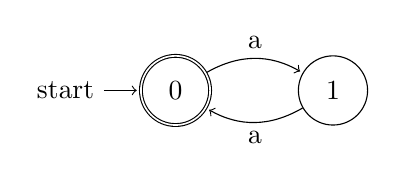
\begin{tikzpicture}[shorten >=1pt,node distance=2cm,on grid,auto] 
  \node[state,initial,accepting] (0) {$0$}; 
  \node[state] (1) [right=of 0] {$1$};
    \path[->] 
    (0) edge [bend left] node {a} (1)
    (1) edge [bend left] node {a} (0);
\end{tikzpicture}
\begin{agda}
dfa-[aa]* = make-dfa 3 0F 2F (0F ∷ []) (
        (0F , a , 1F)
      ∷ (1F , a , 0F)
      ∷ []
    )
\end{agda}
The regular expression \texttt{a*b?a*} can also be defined using three states, where $0$ is the starting state and $2$ is the error state:

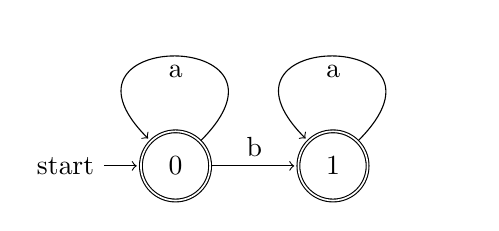
\begin{tikzpicture}[shorten >=1pt,node distance=2cm,on grid,auto] 
  \node[state,initial,accepting] (0) {$0$}; 
  \node[state,accepting] (1) [right=of 0] {$1$};
    \path[->] 
    (0) edge [loop] node {a} (0)
        edge node {b} (1)
    (1) edge [loop] node {a} (1);
\end{tikzpicture}
\begin{agda}
dfa-a*b?a* = make-dfa 3 0F 2F (0F ∷ 1F ∷ []) (
        (0F , a , 0F)
      ∷ (0F , b , 1F)
      ∷ (1F , a , 1F)
      ∷ []
    )
\end{agda}
The implementation for \texttt{a*b*} is very similar to the previous one:

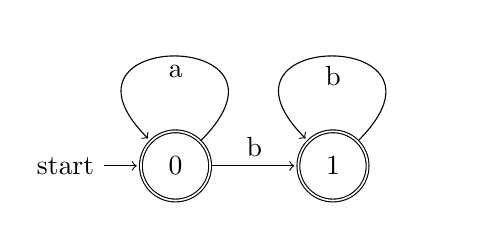
\begin{tikzpicture}[shorten >=1pt,node distance=2cm,on grid,auto] 
  \node[state,initial,accepting] (0) {$0$}; 
  \node[state,accepting] (1) [right=of 0] {$1$};
    \path[->] 
    (0) edge [loop] node {a} (0)
        edge node {b} (1)
    (1) edge [loop] node {b} (1);
\end{tikzpicture}
\begin{agda}
dfa-a*b* = make-dfa 3 0F 2F (0F ∷ 1F ∷ []) (
        (0F , a , 0F)
      ∷ (0F , b , 1F)
      ∷ (1F , b , 1F)
      ∷ []
    )
\end{agda}
For \texttt{(a(c+b))*} we again use three states:

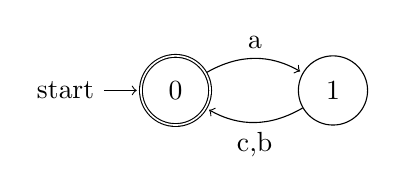
\begin{tikzpicture}[shorten >=1pt,node distance=2cm,on grid,auto] 
  \node[state,initial,accepting] (0) {$0$}; 
  \node[state] (1) [right=of 0] {$1$};
    \path[->] 
    (0) edge [bend left] node {a} (1)
    (1) edge [bend left] node {c,b} (0);
\end{tikzpicture}
\begin{agda}
dfa-[a[c+b]]* = make-dfa 3 0F 2F (0F ∷ []) (
        (0F , a , 1F)
      ∷ (1F , b , 0F)
      ∷ (1F , c , 0F)
      ∷ []
    )
\end{agda}
\subsection{Extended transition function}
The language of a DFA is the set of strings for which the computation from the starting state ends up in a final state. We can express the computation as a function, also known as the extended transition function. It receives a DFA as input, a state, and a string and recursively computes the resulting state based the definition of the $\delta$ function of the DFA:
\begin{agda}
open Dfa

δ^ : ∀{n} → (dfa : Dfa n) → (q : Fin n) → String → Fin n
δ^ dfa q [] = q
δ^ dfa q (x ∷ s) = δ^ dfa (δ dfa q x) s
\end{agda}
Here is a simple property about the extended transition function applied to the concatenation of two strings:
\begin{agda}
lemma-δ^ : ∀{n}
  (dfa : Dfa n)
  → (s : String)
  → (t : String)
  → (q : Fin n)
  → δ^ dfa q (s ++ t) ≡ δ^ dfa (δ^ dfa q s) t
lemma-δ^ dfa [] t q = refl
lemma-δ^ dfa (c ∷ s) t q = lemma-δ^ dfa s t (δ dfa q c)
\end{agda}
\subsection{Language of a DFA}
A string $s$ belongs to the language of a DFA $A$, here denoted as $A ↓ s$, if the extended transition function leads to a final state, beginning at the starting state of $A$. Since the result of the extended transition function is of type \texttt{Fin n} and the subset of final states is of type \texttt{Subset n}, we define the membership relation between strings and DFAs as the membership relation between \texttt{Fin n} and \texttt{Subset n}.\\
As shown previously, the membership relation between \texttt{Fin n} and \texttt{Subset n} is decidable. Therefore, membership between strings and languages of DFAs is also decidable.
\begin{agda}
infix 10 _↓_
_↓_ : ∀{n} → Dfa n → String → Set
dfa ↓ s  = δ^ dfa (S dfa) s ∈ F dfa

_↓?_ : ∀{n} → (dfa : Dfa n) → (s : String) → Dec (dfa ↓ s)
dfa ↓? s = δ^ dfa (S dfa) s ∈? F dfa
\end{agda}
We can immediately tell if a string is accepted or rejected by simply evaluating the result of the extended transition function. For example, the DFA for the regular expression \texttt{(aa)*} accepts \texttt{aa} and rejects string \texttt{aaa}:
\begin{agda}
p0 : dfa-[aa]* ↓ (a ∷ a ∷ [])
p0 = tt

p1 : ¬ dfa-[aa]* ↓ (a ∷ a ∷ a ∷ [])
p1 ()
\end{agda}
Another example is the fact that the DFA for \texttt{a*b?a*} accepts \texttt{aba} and rejects \texttt{bba}:
\begin{agda}
p2 : dfa-a*b?a* ↓ (a ∷ b ∷ a ∷ [])
p2 = tt

p3 : ¬ dfa-a*b?a* ↓ (b ∷ b ∷ a ∷ [])
p3 ()
\end{agda}

\section{Non-deterministic Finite Automata}
Every regular expression can be transformed into a finite state automaton that recognizes the same language (the inverse is also true). Except for the base cases, there are three basic language operations upon which regular expressions are defined: union, concatenation, and star. Implementing these operations using DFAs is rather difficult, so we introduce a new concept of finite state automata: Non-deterministic finite state automata. NFAs might seem more powerful than DFAs, but it can be shown that they are equivalent. In our implementation, we won't use spontaneous transitions, as they could require additional termination proofs.

\subsection{Definition}
The NFA type is similar to the DFA one, except for the transition function which produces a \texttt{Subset n} instead of a single state:
\begin{agda}
record Nfa (n : ℕ) : Set where
  field
    S : Fin n
    δ : Fin n → Σ → Subset n
    F : Subset n
\end{agda}
To simplify the constructions, we define the helper functions \texttt{make-nfa-δ} and \texttt{make-nfa} similarly to the ones used for DFAs, with the addition that the third element of the transitions triples is a list of reached states instead of a single state:
\begin{agda}
NfaTransitionsList = λ n → List (Fin n × Σ × List (Fin n))

make-nfa-δ : ∀{n}
  → Fin n
  → NfaTransitionsList n
  → (Fin n → Σ → Subset n)
make-nfa-δ err [] = λ _ _ → ⁅ err ⁆
make-nfa-δ err ((q , x , ps) ∷ xs)
  = λ h y → if ⌊ q ≟ᶠ h ⌋ ∧ ⌊ x ≟ y ⌋
            then ⋃ (map ⁅_⁆ ps)
            else make-nfa-δ err xs h y

make-nfa : (n : ℕ)
  → Fin n
  → Fin n
  → List (Fin n)
  → NfaTransitionsList n
  → Nfa n
make-nfa n start error finals transitions
  = record
    { S = start
    ; δ = make-nfa-δ error transitions
    ; F = ⋃ (map ⁅_⁆ finals)
    }
\end{agda}
For example, we can implement a NFA accepting the strings of $a$s and $b$s containing the substring $babb$. 

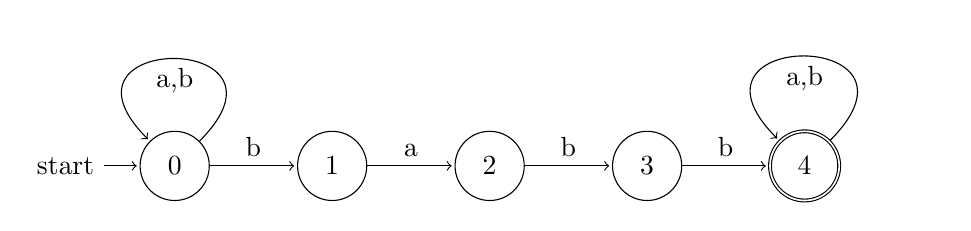
\begin{tikzpicture}[shorten >=1pt,node distance=2cm,on grid,auto] 
  \node[state,initial] (0) {$0$};
  \node[state] (1) [right=of 0] {$1$};
  \node[state] (2) [right=of 1] {$2$};
  \node[state] (3) [right=of 2] {$3$};
  \node[state,accepting] (4) [right=of 3] {$4$};
    \path[->] 
    (0) edge [loop] node {a,b} (0)
        edge node {b} (1)
    (1) edge node {a} (2)
    (2) edge node {b} (3)
    (3) edge node {b} (4)
    (4) edge [loop] node {a,b} (4);
\end{tikzpicture}
\begin{agda}
nfa-babb-substring = make-nfa 6 0F 5F (4F ∷ []) (
        (0F , a , 0F ∷ [])
      ∷ (0F , b , 0F ∷ 1F ∷ [])
      ∷ (1F , a , 2F ∷ [])
      ∷ (2F , b , 3F ∷ [])
      ∷ (3F , b , 4F ∷ [])
      ∷ (4F , a , 4F ∷ [])
      ∷ (4F , b , 4F ∷ [])
      ∷ []
    )
\end{agda}
Another example is the NFA accepting $a$s terminating by $abc$:

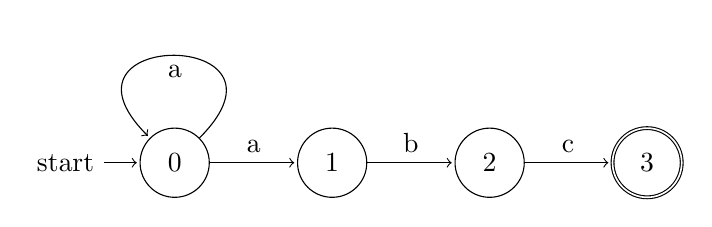
\begin{tikzpicture}[shorten >=1pt,node distance=2cm,on grid,auto] 
  \node[state,initial] (0) {$0$};
  \node[state] (1) [right=of 0] {$1$};
  \node[state] (2) [right=of 1] {$2$};
  \node[state,accepting] (3) [right=of 2] {$3$};
    \path[->] 
    (0) edge [loop] node {a} (0)
        edge node {a} (1)
    (1) edge node {b} (2)
    (2) edge node {c} (3);
\end{tikzpicture}
\begin{agda}
nfa-term-by-abc = make-nfa 5 0F 4F (3F ∷ []) (
        (0F , a , 0F ∷ 1F ∷ [])
      ∷ (1F , b , 2F ∷ [])
      ∷ (2F , c , 3F ∷ [])
      ∷ []
    )
\end{agda}
\subsection{Language}
The \texttt{Subset n} result of the $\delta$ adds the non-determinism. The computation of a NFA is no longer linear, as it proceeds on all the ramifications of the resulting subsets of $\delta$. A string is accepted if the NFA reaches a final state in any of the branches:
\begin{agda}
open Nfa
accepts : ∀{n} → Nfa n → Fin n → String → Bool
accepts A q []       = F A ! q
accepts A q (c ∷ s) 
  = any λ p → (δ A q c) ! p ∧ accepts A p s
\end{agda}
Where \texttt{any} checks if any number of type \texttt{Fin n} satisfies a given function:
\begin{agda}
any : ∀{n} → (P : Fin n → Bool) → Bool
any {zero}  P = false
any {suc _} P = P fzero ∨ any λ x → P (fsuc x)
\end{agda}
A string belongs to the language of a NFA \texttt{A} if \texttt{A} accepts the string beginning at its starting state:
\begin{agda}
_↓_ : ∀{n} → Nfa n → String → Set
A ↓ s  = T (accepts A (S A) s)
\end{agda}
Since \texttt{accepts} is a simple function, the membership relation \texttt{A ↓ s} becomes easily decidable by evaluating the result of \texttt{accepts}:
\begin{agda}
_↓?_ : ∀{n} → (A : Nfa n) → (s : String) → Dec (A ↓ s)
A ↓? s = T? (accepts A (S A) s)
\end{agda}
For example, referring to the NFA \texttt{nfa-babb-substring}, we can show that it accepts the strings $babb$ and $ababbbb$, but rejects the string $aba$:
\begin{agda}
babb : String
babb = b ∷ a ∷ b ∷ b ∷ []

x : nfa-babb-substring ↓ babb
x = tt

y : nfa-babb-substring ↓ (a ∷ babb ++ b ∷ b ∷ [])
y = tt

z : ¬ nfa-babb-substring ↓ (a ∷ b ∷ a ∷ [])
z ()
\end{agda}
Another example is the fact that \texttt{nfa-term-by-abc} accepts the strings $abc$ and $aaaabc$ but rejects the string $bac$:
\begin{agda}
abc : String
abc = a ∷ b ∷ c ∷ []

t : nfa-term-by-abc ↓ (abc)
t = tt

u : nfa-term-by-abc ↓ (a ∷ a ∷ a ∷ abc)
u = tt

v : ¬ nfa-term-by-abc ↓ (b ∷ a ∷ c ∷ [])
v ()
\end{agda}
When a NFA $A$ accepts a non-empty string like $x :: xs$ from a state $q$, we can compute one ``next'' state reached from $q$ with symbol $x$, from which $A$ accepts $xs$: 
\begin{agda}
-- Lemma
anyToExists : ∀{n} {f : Fin n → Bool} 
  → T (any f) 
  → ∃[ i ] T(f i)

nextState : ∀{n x xs q} {nfa : Nfa n}
  → T (accepts nfa q (x ∷ xs))
  → ∃[ p ] ( p ∈ (δ nfa q x)  × T (accepts nfa p xs))
nextState {n} acc-x-xs with anyToExists {n} acc-x-xs
... | p , p∈δqx_∧_acc-p-xs = p , (splitAnd p∈δqx_∧_acc-p-xs)
\end{agda}
Saying that a NFA accepts the empty string is equivalent to saying that its starting state is final:
\begin{agda}
emptyLanguage : ∀{n} {nfa : Nfa n} 
    → nfa ↓ ε ≡ S nfa ∈ F nfa
emptyLanguage = refl
\end{agda}


\subsection{Union}
Given two NFAs $A$ and $B$, we can build a new NFA $C$ whose language is the union of the two: $L(C)$ = $L(A)$ $\cup$ $L(B)$. The number of states of the resulting NFA is the sum of the number of states of the original two, with one additional state. This additional state is also the starting state. 
Given a state $q$ and a symbol $c$, the transition function $\delta (q, c)$ is defined in the following way:
\begin{itemize}
    \item case $q$ is zero (the additional starting state): the resulting subset contains the states reached by $A$ and $B$ from their starting states with the given input symbol $c$
    \item case $q$ is a state of $A$: the resulting subset contains the states reached by $A$ from $q$ with $c$
    \item case $q$ is a state of $B$: the resulting subset contains the states reached by $B$ from $q$ with $c$
\end{itemize}

The final states subset contains the final states of $A$ and $B$ and eventually the new starting state if the empty string belongs to $A$ or $B$.\\
Given two subsets $T$ of size $n$ and $U$ of size $m$, using the vector concatenation function, we can create a subset of size $n+m$ containing distinctly all the elements of $T$ and $U$.\\
We use the previously described function \texttt{splitAt} to determine if a given state of type \texttt{Fin (1 + n + m)} is the additional state, a state of $A$ or a state of $B$.

\begin{agda}
union : ∀{n m} → Nfa n → Nfa m → Nfa (1 + n + m)
union {n} {m} A B =
  record
    { S = fzero
    ; δ = d
    ; F = sf ++ (F A) ++ (F B)
    }
  where
    d : Fin (1 + n + m) → Σ → Subset (1 + n + m)
    d q c  with splitAt 1 q
    d q c | inj₁ z = ∅ {1} ++ (δ A (S A) c) ++ (δ B (S B) c)
    d q c | inj₂ f with splitAt n f
    ... | inj₁ l = ∅ {1} ++ (δ A l c) ++ ∅
    ... | inj₂ r = ∅ {1} ++ ∅ ++ (δ B r c)

    sf : Subset 1
    sf with A ↓? ε | B ↓? ε
    sf | no ε∉l | no ε∉r = ∅
    sf | _     | _       = FullSet
\end{agda}
For example, we can build the union of the two NFAs previously introduced and we can show it accepts $abc$ and $babb$ but rejects $bac$:
\begin{agda}
nfa-union-babb-abc = union nfa-babb-substring nfa-term-by-abc

q : nfa-union-babb-abc ↓ (abc)
q = tt

r : nfa-union-babb-abc ↓ (b ∷ a ∷ b ∷ b ∷ [])
r = tt

s : ¬ nfa-union-babb-abc ↓ (b ∷ a ∷ c ∷ [])
s ()
\end{agda}
Before proving that the construction is correct, we first need to prove that the two NFAs are still present in the new NFA after the construction. We show this by proving that both NFAs individually accept a string from a state if and only if they accept it from the same state relatively injected/raised into the union.\\
The proofs are by induction on the string. For the NFA provided as first argument, the relative state is injected:
\begin{agda}
union-preservesˡ : ∀{n m} {A : Nfa n} {B : Nfa m} {q : Fin n}
  → (s : String)
  → T (accepts A q s)
    ⇔
    T (accepts (union A B) (fsuc (inject+ m q)) s)
union-preservesˡ {n}{m} {A} {B} {q} s =
  record { to = to s q ; from = from s q }
  where
  to : (s : String) (q : Fin n)
    → T (accepts A q s)
    → T (accepts (union A B) (fsuc (inject+ m q)) s)
  to [] q acc with
      A ↓? ε
    | B ↓? ε
    | ++-inject (F A) (F B) q acc
  ...| yes _ | yes _ | v = v
  ...| yes _ | no  _ | v = v
  ...| no  _ | yes _ | v = v
  ...| no  _ | no  _ | v = v
  to (c ∷ s) q acc with nextState {_} {c} {s} acc
  ... | w , w∈δqc , t rewrite splitAt-inject+ n m q
                  with to s w t
                  | ++-inject {n}{m} (δ A q c) ∅ w w∈δqc
  ... | z | d = fromExists (inject+ m w , (joinAnd d z))

  from : (s : String) (q : Fin n)
    → T (accepts (union A B) (fsuc (inject+ m q)) s)
    → T (accepts A q s)
  from [] q d rewrite
        sym (lookup-++ˡ (F A) (F B) q)
    with A ↓? ε | B ↓? ε
  ... | yes _ | yes _  = d
  ... | yes _ | no  _  = d
  ... | no  _ | yes _  = d
  ... | no  _ | no  _  = d
  from (x ∷ s) q d with nextState {_} {x} {s} {fsuc (inject+ m q)} d
  ... | w , w∈δqx , accWs rewrite splitAt-inject+ n m q 
    with q∈ss++∅ w (δ A q x) w∈δqx
  ... | p , eq , ds rewrite eq =
    fromExists (p , joinAnd ds (from s p accWs))
\end{agda}
For the NFA provided as second argument, the proof is essentially the same and we only list its statement:
\begin{agda}
union-preservesʳ : ∀{n m} {A : Nfa n} {B : Nfa m} {q : Fin m}
  → (s : String)
  → T (accepts B q s)
    ⇔
    T (accepts (union A B) (fsuc (raise n q)) s)
\end{agda}
We now show that a string belongs to the language of the union if and only if it belongs to the language of the first or the second NFA.\\
The proof is by induction on the string as a consequence of \texttt{union-preserves$^l$} and \texttt{union-preserves$^r$}:
\begin{agda}
union-correct : ∀{n m : ℕ} {A : Nfa n} {B : Nfa m}
  → (s : String)
  → A ↓ s ⊎ B ↓ s ⇔ union A B ↓ s
union-correct {n}{m}{A}{B} s =
  record { to = to s ; from = from s }
  where
  to : (s : String) → A ↓ s ⊎ B ↓ s → union A B ↓ s
  to [] ac with A ↓? ε | B ↓? ε
  ... | yes _  | yes _ = tt
  ... | yes _  | no  _ = tt
  ... | no  _  | yes _ = tt
  ... | no ¬p  | no ¬q = ⊥-elim ((¬p ¬-⊎ ¬q) ac)

  to (c ∷ s) (inj₁ A↓cs) with nextState {_} {c} {s} A↓cs
  ... | w , w∈δA , accepts-s-w-A
                with ++-inject (δ A (S A) c) (δ B (S B) c) w w∈δA
                   | _⇔_.to (union-preservesˡ s) accepts-s-w-A
  ... | w∈δA∪B | accepts-s-w-A∪B
    = fromExists (inject+ m w , joinAnd w∈δA∪B accepts-s-w-A∪B)

  to (c ∷ s) (inj₂ B↓cs) with nextState {_} {c} {s} B↓cs
  ... | w , w∈δB , accepts-w-B
                with ++-raise (δ A (S A) c) (δ B (S B) c) w w∈δB
                   | _⇔_.to (union-preservesʳ s) accepts-w-B
  ... | w∈δA∪B | accepts-s-w-A∪B
    = fromExists (raise n w , joinAnd w∈δA∪B accepts-s-w-A∪B)


  from : (s : String) → union A B ↓ s → A ↓ s ⊎ B ↓ s
  from [] d with A ↓? ε | B ↓? ε
  ... | yes p | yes p₁ = inj₁ p
  ... | yes p | no ¬p  = inj₁ p
  ... | no ¬p | yes p  = inj₂ p

  from (x ∷ s) d with nextState {suc n + m} {x} {s} {0F} d
  ... | w , w∈δSc , accepts-w-s 
    with split-∈++ w (δ A (S A) x) (δ B (S B) x) w∈δSc
  ... | inj₁ (p , eq , z) rewrite eq =
    inj₁ (fromExists (
      p , joinAnd z (_⇔_.from (union-preservesˡ s) accepts-w-s)))
  ... | inj₂ (p , eq , z) rewrite eq =
    inj₂ (fromExists (
      p , joinAnd z (_⇔_.from (union-preservesʳ s) accepts-w-s)))
\end{agda}
\subsection{Concatenation}
The concatenation function is similar to the union. We add a new starting state and build the transition function based on the transition functions of the input NFAs.\\
Given $q$ and $c$, $\delta (q, c)$ is defined as follows:
\begin{itemize}
    \item case $q$ is zero (the additional starting state): 
        \begin{itemize}
            \item if $\epsilon \not \in L(A)$: the resulting subset contains only states reached by $A$ from its starting state with symbol $c$
            \item if $\epsilon \in L(A)$: the resulting subset contains the states reached by both NFA from their starting state with symbol $c$
        \end{itemize}
    \item case $q$ is a state of A: 
        \begin{itemize}
            \item if $q$ is not final: the resulting subset is the subset of states reached by $A$ from $q$ with the symbol $c$
            \item otherwise: in addition to the previous case subset we also add the states reached by $B$ from its starting state with the symbol $c$
        \end{itemize}
    \item case $q$ is a state of $B$: the result is the subset of states reached by B from $q$ with the symbol $c$
\end{itemize}
The final states subset is defined as:
\begin{itemize}
    \item if $\epsilon$ belongs to neither $L(A)$ nor $L(B)$: only the final states of $B$ are final
    \item if $\epsilon$ belongs to both $L(A)$ and $L(B)$: the starting state is final along with the final states of $A$ and $B$
    \item if $\epsilon$ belong to $L(B)$ but does not belong to $L(A)$: only the final states of $A$ and $B$ are final
\end{itemize}
And here is the implementation in Agda:
\begin{agda}
concat : ∀{n m} → Nfa n → Nfa m → Nfa (1 + n + m)
concat {n} {m} A B =
  record
    { S = fzero
    ; δ = d
    ; F = f
    }
  where
    d : Fin (1 + n + m) → Σ → Subset (1 + n + m)
    d q c with splitAt 1 q
    d _ c | inj₁ z with A ↓? ε
    ... | yes isf = ∅ {1} ++ (δ A (S A) c) ++ (δ B (S B) c)
    ... | no ¬isf = ∅ {1} ++ (δ A (S A) c) ++ ∅
    d _ c | inj₂ mn with splitAt n mn
    d _ c | inj₂ mn | inj₁ l with l ∈? F A
    ... | yes isf = ∅ {1} ++ (δ A l c) ++ (δ B (S B) c)
    ... | no ¬isf = ∅ {1} ++ (δ A l c) ++  ∅
    d _ c | inj₂ mn | inj₂ r = ∅ {1} ++ ∅ ++ (δ B r c)

    f : Subset (1 + n + m)
    f with A ↓? ε | B ↓? ε
    f | yes ε∈l | yes ε∈r = FullSet {1} ++ F A ++ F B
    f | no ε∉l | yes ε∈r = ∅ {1} ++ F A ++ F B
    f | _ | no ε∉r = ∅ {1} ++ ∅ ++ F B
\end{agda}
For example, we can apply this function to our two NFAs and concatenate \texttt{nfa-babb-substring} on the left of \texttt{nfa-term-by-abc}. We can show that the concatenation accepts \texttt{babbabc} but rejects \texttt{babb}, because the NFA \texttt{nfa-term-by-abc} is on the right and requires a string terminating by \texttt{abc}:
\begin{agda}
nfa-concat-babb-abc = concat nfa-babb-substring nfa-term-by-abc

o : nfa-concat-babb-abc ↓ (babb ++ abc)
o = tt

p : ¬ nfa-concat-babb-abc ↓ babb
p ()
\end{agda}
The correctness proofs follow the same techniques used for the union. We first show that the two NFAs are preserved in the concatenation after the construction. Then we conclude that a string $s$ belongs to the concatenation if and only if it can be divided into two strings $u,v$ such that $u$ belongs to $L(A)$ and $v$ belongs to $L(B)$. Here are the statements of these properties:
\begin{agda}
concat-preservesʳ : ∀{n m : ℕ} {p} {A : Nfa n} {B : Nfa m}
  → (v : String)
  → T(accepts B p v)
    ⇔
    T(accepts (concat A B) (raise 1 (raise n p)) v)
    
concat-preservesˡ : ∀{n m : ℕ} {q} {A : Nfa n} {B : Nfa m}
  → (s : String)
  → T(accepts (concat A B) (fsuc (inject+ m q)) s)
    ⇔
    ∃[ u ] ∃[ v ] (s ≡ u ++ˢ v × T(accepts A q u) × B ↓ v)

concat-correct : ∀{n m : ℕ} {A : Nfa n} {B : Nfa m}
  → (s : String)
  → concat A B ↓ s
    ⇔
    ∃[ u ] ∃[ v ] (s ≡ u ++ˢ v × A ↓ u × B ↓ v)
\end{agda}
\subsection{Star}
Given a NFA $A$ with $n$ states, we can define the star operation by adding one single state. It is the new starting state and it is also final, as the empty string always belongs to the star closure. The transition function $\delta(q, c)$ is defined as follows:
\begin{itemize}
    \item if $q$ is the additional state: the result is the subset of states reached by $A$ from its starting state with symbol $c$
    \item otherwise, $q$ is one of the states of $A$:
    \begin{itemize}
        \item if $q$ is final: the resulting subset contains the states reached by $A$ with symbol $c$ from both $q$ and its starting state
        \item otherwise: the result is simply the subset of states reached by $A$ from $q$ with $c$
    \end{itemize}
\end{itemize}
\begin{agda}
star : ∀{n} → Nfa n → Nfa (1 + n)
star {n} nfa =
  record { S = fzero ; δ = d ; F = ⁅ fzero ⁆ ++ F nfa }
  where
    d : Fin (1 + n) → Σ → Subset (1 + n)
    d q c with splitAt 1 q
    d _ c | inj₁ z = ∅ ++ δ nfa (S nfa) c
    d _ c | inj₂ p with p ∈? F nfa
    ... | yes isf = ∅ ++ (δ nfa (S nfa) c) ∪ (δ nfa p c)
    ... | no ¬isf = ∅ ++ δ nfa p c
\end{agda}
For example, we can show that the \texttt{star} construction of \texttt{nfa-term-by-abc} accepts the strings $abcabc$ and $abcaaabc$ but rejects $abccc$:
\begin{agda}
k : nfa-star-term-abc ↓ (abc ++ abc)
k = tt

l : nfa-star-term-abc ↓ (abc ++ a ∷ a ∷ abc)
l = tt

m : ¬ nfa-star-term-abc ↓ (abc ++ c ∷ c ∷ [])
m ()
\end{agda}
Again, we first show that the original NFA is preserved after the star construction and then conclude with the correctness. However, in this case, we have two separate proofs, as the empty string always belongs to the star construction but might not be accepted by the original NFA. Here are the statements:
\begin{agda}
star-preserves : ∀{n} {nfa} {q : Fin n} {s}
  → T(accepts (star nfa) (fsuc q) s)
    ⇔
    ∃[ u ] ∃[ v ] (
          s ≡ u ++ˢ v 
        × T(accepts nfa q u) 
        × star nfa ↓ v)

star-correct1 : ∀{n} {s v : String} {nfa : Nfa n}
  → nfa ↓ s × (star nfa) ↓ v
  → (star nfa) ↓ (s ++ˢ v)
 
star-correct2 : ∀{n} {a} {s : String} {nfa : Nfa n}
  → (star nfa) ↓ (a ∷ s)
  → ∃[ u ] ∃[ v ](
          s ≡ u ++ˢ v 
        × nfa ↓ (a ∷ u) 
        × star nfa ↓ v)
\end{agda}
\section{Deciding RegExp membership using NFAs}
\subsection{NFAs for $L(\varnothing)$, $L(\{\epsilon\})$, $L(\{c\})$}
Before diving into the generation of a NFA from a regular expression, we first define the NFAs for the base cases: $L(\varnothing)$, $L(\{\epsilon\})$, $L(\{c\})$.\\
For the empty language, we use one single state which is the starting state and it is not final:
\begin{agda}
nfa-∅ : Nfa 1
nfa-∅ = record { S = 0F ; δ = λ _ _ → ⁅ 0F ⁆ ; F = ∅ }

nfa-∅-is-empty : (s : String) → ¬ (nfa-∅ ↓ s)
nfa-∅-is-empty (x ∷ s) r = ⊥-elim (nfa-∅-is-empty s (extractOrL r))
\end{agda}
The language with just the empty string has two states. The starting state which is final and an error state where all transitions end up:
\begin{agda}
nfa-ε : Nfa 2
nfa-ε = record { S = 0F ; δ = λ _ _ → ⁅ 1F ⁆ ; F = ⁅ 0F ⁆ }

1F-is-error : (s : String) → ¬ (T (accepts nfa-ε 1F s))
1F-is-error [] z = z
1F-is-error (x ∷ s) z = ⊥-elim (1F-is-error s (extractOrL z))

nfaε-correct : (s : String) → ¬ (s ≡ ε) → ¬ (nfa-ε ↓ s)
nfaε-correct [] a b = a refl
nfaε-correct (x ∷ s) a b = 1F-is-error s (extractOrL b)
\end{agda}
The language with just a single character string has three states. The construction is defined based on an input character $c$. The first state is the starting state. The second state is the only final state. The third state is an error state. There is only one transition with character $c$ from the starting state leading to the second state. All other transitions end up in the error state:
\begin{agda}
nfa-c : (c : Σ) → Nfa 3
nfa-c c = record { S = 0F ; δ = δ ; F = ⁅ 1F ⁆ }
  where
    δ : Fin 3 → Σ → Subset 3
    δ 0F k with k ≟ c
    ... | yes p = ⁅ 1F ⁆
    ... | no ¬p = ⁅ 2F ⁆
    δ _ _ = ⁅ 2F ⁆

2F-is-error : ∀{c s} → ¬ (T (accepts (c-nfa c) 2F s ))
2F-is-error {c} {x ∷ s} d =
  contradiction (extractOrL d) (2F-is-error {c} {s})

nfac-correct : ∀{c}{s} → nfa-c c ↓ s → s ≡ (c ∷ [])
nfac-correct {c} {x ∷ []} d with x ≟ c
... | yes p = cong (_∷ []) p
nfac-correct {c} {x ∷ y ∷ s} d with x ≟ c
... | yes p = contradiction d (2F-is-error {c} {x ∷ y ∷ s})
... | no ¬p = contradiction d (2F-is-error {c} {x ∷ y ∷ s})
\end{agda}

\subsection{Regular expressions to NFAs}
We now prove that for every regular expression there is a NFA which recognizes the same language.\\
For ⟨⟩, the equivalent NFA is \texttt{nfa-∅}.\\
For ⟨ε⟩, the equivalent NFA is \texttt{nfa-ε}.\\
For \texttt{Atom c}, we build \texttt{nfa-c} passing \texttt{c}.\\
For \texttt{(R + S)}, using \texttt{union}, we build the union of the two NFAs generated inductively based on \texttt{R} and \texttt{S}.\\
For \texttt{(R · S)}, using \texttt{concat}, we build the concatenation of the two NFAs generated inductively based on \texttt{R} and \texttt{S}.\\
For \texttt{R *}, using \texttt{star}, we build the star closure of the NFA generated inductively based on \texttt{R}.\\
We conclude that a string belongs to the language of a regular expression if and only if the generated NFA accepts it, as a consequence of the correctness proofs \texttt{nfa-∅-is-empty}, \texttt{nfaε-correct}, \texttt{nfac-correct}, \texttt{union-correct}, \texttt{concat-correct},\\ \texttt{star-correct2} and \texttt{star-correct1}:
\begin{agda}
toNFA : (R : RegExp)
    → ∃₂ λ (n : ℕ) (nfa : Nfa n)
      → ∀ (s : String)
      → s ∈ R ⇔ nfa ↓ s
toNFA ⟨⟩ = 1 , nfa-∅ , λ s → record
    { to = λ ()
    ; from = λ nfa↓s → ⊥-elim (nfa-∅-is-empty s nfa↓s)
    }

toNFA ⟨ε⟩ = 2 , nfa-ε , iff
  where
  iff : (s : String)
    → s ∈ ⟨ε⟩ ⇔ nfa-ε ↓ s
  iff [] = record { to = λ _ → tt ; from = λ _ → in-ε }
  iff (x ∷ s) = record
    { to = λ ()
    ; from = λ nfa↓xs → ⊥-elim (nfaε-correct (x ∷ s) (λ ()) nfa↓xs )
    }

toNFA (Atom c) = 3 , nfa-c c , λ s → to IFF from
  where
  to : ∀{s}
    → s ∈ Atom c
    → nfa-c c ↓ s
  to (in-c c) with c ≟ c
  ... | yes p = tt
  ... | no ¬p = ¬p refl

  from : ∀{s}
    → nfa-c c ↓ s
    → s ∈ Atom c
  from {s} nfa↓s rewrite nfac-correct {c} {s} nfa↓s = in-c c

toNFA (R + F) with toNFA R | toNFA F
... | n , A , w∈R⇔A↓w | m , B , w∈F⇔B↓w =
  suc n ℕ.+ m , union A B , λ s → to s IFF (from s)
  where
  to :  (s : String)
    → s ∈ (R + F)
    → union A B ↓ s
  to s (in+l s∈R)
    = _⇔_.to (union-correct s) (inj₁ (_⇔_.to (w∈R⇔A↓w s) s∈R))
  to s (in+r s∈F)
    = _⇔_.to (union-correct s) (inj₂ (_⇔_.to (w∈F⇔B↓w s) s∈F))

  from : (s : String)
    → union A B ↓ s
    → s ∈ (R + F)
  from s A∪B↓s with _⇔_.from (union-correct s) A∪B↓s
  ...| inj₁ A↓s = in+l (_⇔_.from (w∈R⇔A↓w s) A↓s)
  ...| inj₂ B↓s = in+r (_⇔_.from (w∈F⇔B↓w s) B↓s)

toNFA (R · F) with toNFA R | toNFA F
... | n , A , w∈R⇔A↓w | m , B , w∈F⇔B↓w =
  suc n ℕ.+ m , concat A B , λ s → to s IFF (from s)
  where
  to : (s : String)
    → s ∈ (R · F)
    → concat A B ↓ s
  to _ (in-· {u} {v} u∈R v∈F) =
    _⇔_.from (concat-correct (u ++ˢ v))
      (u
      , v
      , refl
      , _⇔_.to (w∈R⇔A↓w u) u∈R
      , _⇔_.to (w∈F⇔B↓w v) v∈F)

  from : (s : String)
    → concat A B ↓ s
    → s ∈ (R · F)
  from s AB↓s with _⇔_.to (concat-correct s) AB↓s
  ... | u , v , s≡uv , A↓u , B↓v rewrite s≡uv =
    in-· (_⇔_.from (w∈R⇔A↓w u) A↓u) (_⇔_.from (w∈F⇔B↓w v) B↓v)

toNFA (R *) with toNFA R
... | n , A , s∈R⇔A↓s =
  suc n , star A , λ s → (to s) IFF (from s)
  where
  to : (s : String)
    → s ∈ (R *)
    → star A ↓ s
  to _ in-*1 = tt
  to _ (in-*2 {u} {v} u∈R v∈R*) =
    star-correct1 {_} {u} {v} (_⇔_.to (s∈R⇔A↓s u) u∈R , (to v v∈R*))

  lenv<lenau++v : ∀{u v} → (a : Σ) → length v <′ length (a ∷ u ++ˢ v)
  lenv<lenau++v {[]} {v} a = ≤′-refl
  lenv<lenau++v {u ∷ us} {v} a = ≤′-step (lenv<lenau++v u)

  star-from-WF : (s : String)
    → star A ↓ s
    → Acc _<′_ (length s)
    → s ∈ (R *)
  star-from-WF [] _ _ = in-*1
  star-from-WF (a ∷ s) A*↓as (acc go) with star-correct2 a s A*↓as
  ... | u , v , as≡uv , A↓au , A*↓v rewrite as≡uv =
    in-*2 (_⇔_.from (s∈R⇔A↓s (a ∷ u)) A↓au)
        (star-from-WF v A*↓v (go (length v) (lenv<lenau++v a)))

  from : (s : String)
    → star A ↓ s
    → s ∈ (R *)
  from s A*↓s = star-from-WF s A*↓s (<′-wellFounded (length s))
\end{agda}
\subsection{Decidable}
The previous result is not just a theorem. It produces a perfectly well-defined NFA which accepts the same language of a given regular expression. We can use it to decide whether or not a string $v$ belongs to $L(F)$.\\
Given a regular expression, we generate the equivalent NFA, compute the result and return to the regular expressions membership relation with the ``⇔'' roperty:
\begin{agda}
_∈?_ : (v : String) → (F : RegExp) → Dec (v ∈ F)
v ∈? F with toNFA F
... | _ , A , v∈F⇔A↓v with A ↓? v
... | yes A↓v = yes (_⇔_.from (v∈F⇔A↓v v) A↓v)
... | no ¬A↓v = 
  no λ v∈F → contradiction (_⇔_.to (v∈F⇔A↓v v) v∈F) ¬A↓v
\end{agda}
For example, by evaluating the expression \texttt{aabaa ∈? a*b?a*}, Agda provides the following membership proof: 
\begin{agda}
yes
  (in-·
     (in-· (in-*2 (in-c a) (in-*2 (in-c a) in-*1)) 
       (in+l (in-c b)))
     (in-*2 (in-c a) 
       (in-*2 (in-c a) (in-*2 (in-c a) in-*1))))
\end{agda}
This approach does the same job as the derivatives one previously described. However, in this case, the generated NFA can be reused multiple times for the same regular expressions. Furthermore, it can be transformed into a deterministic automaton that would have a linear time complexity match.


\section{Pumping Lemma and a Non-regular Langauge}
In this section, we present the Pumping Lemma, a property that holds for any finite state automaton. It can be used to prove that a language is not regular. In fact, we present a simple context-free language which is not recognizable by any finite state automaton. We go back to determinism and use DFAs instead of NFAs to simplify the proofs, but as mentioned, these computation models are equivalent and so they both respect this property.

\subsection{Path}
As hinted, we will use the pigeonhole principle and we will apply it to the path of visited states. Given a string \texttt{s} and a DFA \texttt{A} with \texttt{m} states, we define a function which computes the path of visited states during the execution of \texttt{A} with \texttt{s} as input. The path is a vector of \texttt{Fin m} elements of size equal to the length of \texttt{s}. We only consider past states, so when the string is empty, the list of past states is empty.
\begin{agda}
path : ∀{m} → Dfa m 
    → Fin m 
    → (s : String) 
    → Vec (Fin m) (length s)
path A q [] = []
path A q (c ∷ s) = q ∷ (path A (δ A q c) s)
\end{agda}
We can prove a simple lemma which states that the state at an index \texttt{i} in the path is equal to the state computed by the extended transition function executed with a prefix of length \texttt{i} of the string:
\begin{agda}
lemmaPath : ∀{m}
  → (dfa : Dfa m)
  → (s : String)
  → (i : Fin (length s))
  → (q : Fin m)
  → path dfa q s ! i ≡ δ^ dfa q (take (toℕ i) s)
lemmaPath dfa (c ∷ s) fzero q = refl
lemmaPath dfa (c ∷ s) (fsuc i) q = lemmaPath dfa s i (δ dfa q c)
\end{agda}

\subsection{Power}
A string elevated to the power of \texttt{n} is its self-concatenation \texttt{n} times. We define it recursively based on the exponent:
\begin{agda}
_^_ : String → ℕ → String
s ^ zero = []
s ^ (suc n) = s ++ s ^ n
\end{agda}
For example, the string \texttt{abc} elevated to the power of \texttt{2} generates \texttt{abcabc}.\\
The power operation has some interesting properties, similar to the ones about natural numbers.\\
For example, $s^ns^m$ is equal to $s^{n+m}$:
\begin{agda}
^-join-+ : (s : String) (n m : ℕ)
  → (s ^ n) ++ (s ^ m) ≡ s ^ (n + m)
^-join-+ s 0F     0F = refl
^-join-+ s 0F     (suc m) = refl
^-join-+ s (suc n) m rewrite
      ++-assoc s (s ^ n) (s ^ m)
    | sym (^-join-+ s n m) = refl
\end{agda}
Another example is that $(s^n)^m$ is equal to $s^{n * m}$:
\begin{agda}
^-join-* : (s : String) (n m : ℕ)
  → (s ^ n) ^ m ≡ s ^ (n * m)
^-join-* s 0F 0F = refl
^-join-* s 0F (suc m) = ^-join-* s 0F m
^-join-* s (suc n) 0F = ^-join-* s n 0F
^-join-* s (suc n) (suc m) rewrite
            ^-join-* s (suc n) m
          | ++-assoc s (s ^ n) (s ^ (m + n * m))
          | ^-join-+ s n (m + n * m)
          | *-comm n (suc m)
          | *-comm m n
          | sym (+-assoc n m (n * m))
          | sym (+-assoc m n (n * m))
          | +-comm m n = refl
\end{agda}
\subsection{Pigeonhole principle}
The pigeonhole principle states that given two sets $A$, $B$ and a function $f : A \rightarrow B$, if $B$ has less elements than $A$ then there are at least two distinct elements $i,j$ in $A$ such that $f(i) \equiv f(j)$.\\
In Agda, finite sets can be easily described using the \texttt{Fin n} type, and so the pigeonhole proof makes use of this type. The proof can be found in the standard library of Agda. Here is its statement:
\begin{agda}
pigeonhole : ∀ {m n} → m < n → (f : Fin n → Fin m) →
             ∃₂ λ i j → i ≢ j × f i ≡ f j
\end{agda}
We apply the pigeonhole principle to vectors. Given a vector of size \texttt{m} containing elements of type \texttt{Fin n}, if \texttt{n < m} then there are at least two distinct indexes which point to equal elements. We obtain the following property:
\begin{agda}
pigeonholeVec : ∀{n m}
  → (vec : Vec (Fin n) m)
  → n < m
  → ∃[ i ] ∃[ j ] (
          i <ᶠ j 
        × toℕ j ≤ n 
        × vec ! i ≡ vec ! j)
\end{agda}
We will use these indexes to divide a given string into three substrings. Here we define a lemma about this operation. Given a string $s$ and two numbers $i,j$ such that $i < j \leq |s|$, we can divide $s$ in three substrings $x$, $y$, $z$ which respect the following constraints:
\begin{itemize}
    \item $x$ is the prefix of $s$ of length $i$
    \item $y$ is not empty
    \item $xy$ is the prefix of $s$ of length $j$  
\end{itemize}
Here is the statement:
\begin{agda}
tripartition : (s : String)
  → (i j : Fin (length s))
  → i <ᶠ j
  → ∃[ x ] ∃[ y ] ∃[ z ] (
        s ≡ x ++ y ++ z
      × y ≢ []
      × x ≡ take (toℕ i) s
      × (x ++ y) ≡ take (toℕ j) s
      × length (x ++ y) ≡ toℕ j
    )
\end{agda}

\subsection{Returning to same state}
When a DFA starts at $q$ and returns to $q$ after running a string $s$, then it always returns to the same state for any power of $s$. We show that if δ\texttt{\^}$(q, s) \equiv q$, then for any number $m$, we have that δ\texttt{\^}$(q, s ^ m) \equiv q$: 
\begin{agda}
returns-back : ∀{n}
  → (dfa : Dfa n)
  → (s : String)
  → (q : Fin n)
  → q ≡ δ^ dfa q s
  → ∀(m : ℕ) → q ≡ δ^ dfa q (s ^ m)
returns-back dfa s q eq zero = refl
returns-back dfa s q eq (suc m) with
  returns-back dfa s q eq m | lemma-δ^ dfa s (s ^ m) q
... | ind | lm2 rewrite sym eq = trans ind (sym lm2)
\end{agda}
We extend \texttt{returns-back} lemma by adding a prefix and a suffix and beginning at the starting state:
\begin{agda}
pumping-same-state : ∀{n} {dfa : Dfa n}
  → (s : String)
  → (t : String)
  → (u : String)
  → let p = δ^ dfa (S dfa) s in
     p ≡ δ^ dfa p t
  → dfa ↓ (s ++ t ++ u)
  → ∀ (m : ℕ) → dfa ↓ (s ++ t ^ m ++ u)
pumping-same-state {n} {dfa} s t u p≡δ^pt dfa↓stu m with
  returns-back dfa t (δ^ dfa (S dfa) s) p≡δ^pt m
... | pump with   lemma-δ^ dfa (s ++ t)       u       (S dfa)
                | lemma-δ^ dfa s              (t ^ m) (S dfa)
                | lemma-δ^ dfa s              t       (S dfa)
                | lemma-δ^ dfa (s ++ (t ^ m)) u       (S dfa)
... | d1 | d2 | d3 | d4 rewrite
                  trans pump (sym d2)
                | sym (trans p≡δ^pt (sym d3))
                | ++-assoc s t u
                | ++-assoc s (t ^ m) u
                | trans d1 (sym d4) = dfa↓stu
\end{agda}

\subsection{Pumping Lemma}
Given a DFA $A$ with $m$ states, there exists a number $n$ such that, for every string $w \in L(A)$, if $|w|>n$ then $w$ can be divided into three substrings $x,y,z$ such that:
\begin{itemize}
    \item $w \equiv xyz$
    \item $y \not \equiv \epsilon$
    \item $|xy| \leq n$
    \item $\forall k: xy^kz \in L(A)$
\end{itemize}
One $n$ for which we can be sure this property holds is simply $m$, the number of states of the DFA.\\
We use the \texttt{pigeonholeVec} principle applied to the path. Then we use the computed indexes to divide the string with \texttt{tripartition} which generates the strings $x$, $y$ and $z$ such that $y \not \equiv \epsilon$ and $|xy| \leq m$. \\
The \texttt{pigeonholeVec} also tells us that there are two repeated states in two different positions in the path which correspond exactly at the end of the computation of $x$ and the end of the computation of $y$. In fact, with \texttt{lemmaPath} we obtain that: $\delta$\texttt{\^}$(S, x) \equiv q$ and $\delta$\texttt{\^}$(q, y) \equiv q$.\\
Since $\delta$\texttt{\^}$(q, z) \in F$, using \texttt{pumping-same-state} we conclude that $\forall k: xy^kz \in L(A)$:
\begin{agda}
pumpingLemma : {m : ℕ}
  → (dfa : Dfa m)
  → ∃[ n ] (
    ∀(w : String)
    → dfa ↓ w
    → n < length w
    → ∃[ x ] ∃[ y ] ∃[ z ] (
        w ≡ x ++ y ++ z
        × y ≢ ε
        × length (x ++ y) ≤ n
        × ∀(k : ℕ) → dfa ↓ (x ++ y ^ k ++ z)
      )
  )
pumpingLemma {m} dfa = m , base
  where
  base : ∀(w : String)
    → dfa ↓ w
    → m < length w
    → ∃[ x ] ∃[ y ] ∃[ z ] (
        w ≡ x ++ y ++ z
        × y ≢ []
        × length (x ++ y) ≤ m
        × ∀(k : ℕ) → dfa ↓ (x ++ y ^ k ++ z)
      )
  base w dfa↓w m<len_w with
        pigeonholeVec (path dfa (S dfa) w) m<len_w
  ... | i , j , i<j , j≤n , eq  with
        tripartition w i j i<j
  ... | x , y , z , w≡xyz , y≢ε , x≡takeI , xy≡takeJ , len_xy≡J with
        lemmaPath dfa w i (S dfa) | lemmaPath dfa w j (S dfa)
  ... | lp1 | lp2 rewrite
        sym x≡takeI | sym xy≡takeJ | sym eq | sym len_xy≡J | w≡xyz =
    x , y , z , ( refl , y≢ε , j≤n
        , pumping-same-state x y z
            (trans (sym lp1) (trans lp2 (lemma-δ^ dfa x y (S dfa))))
            dfa↓w
      )
\end{agda}
For example, we can define a DFA accepting binary strings representing multiples of $5$ and then find a substring that can be repeated indefinitely and still preserve the multiple property. The DFA has $6$ states where $0$ is the starting state and $5$ is the error state:

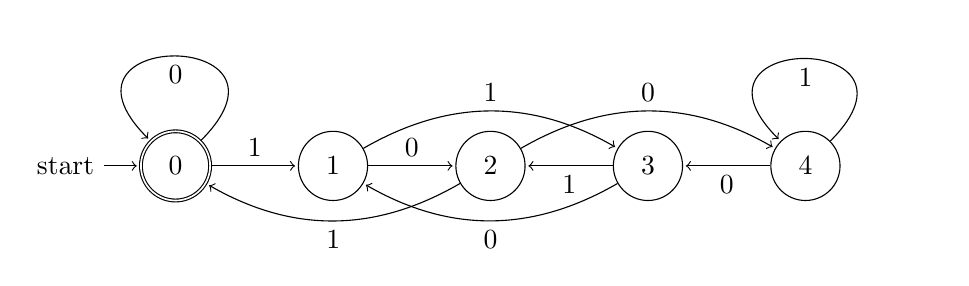
\begin{tikzpicture}[shorten >=1pt,node distance=2cm,on grid,auto] 
  \node[state,initial,accepting] (0) {$0$};
  \node[state] (1) [right=of 0] {$1$};
  \node[state] (2) [right=of 1] {$2$};
  \node[state] (3) [right=of 2] {$3$};
  \node[state] (4) [right=of 3] {$4$};
    \path[->] 
    (0) edge [loop] node {0} (0)
        edge node {1} (1)
    (1) edge node {0} (2)
        edge [bend left] node {1} (3)
    (2) edge [bend left] node {0} (4)
        edge [bend left] node {1} (0)
    (3) edge [bend left] node {0} (1)
        edge node {1} (2)
    (4) edge node {0} (3)
        edge [loop] node {1} (4);
\end{tikzpicture}
\begin{agda}
dfa-binary-multiples-5 = make-dfa 6 0F 5F (0F ∷ []) (
        (0F , 0 , 0F)
      ∷ (0F , 1 , 1F)
      ∷ (1F , 0 , 2F)
      ∷ (1F , 1 , 3F)
      ∷ (2F , 1 , 0F)
      ∷ (2F , 0 , 4F)
      ∷ (3F , 1 , 2F)
      ∷ (3F , 0 , 1F)
      ∷ (4F , 1 , 4F)
      ∷ (4F , 0 , 3F)
      ∷ []
    )
\end{agda}
When we apply the pumping lemma on it with the string $1110011$, which is equal to $115$ base-ten, we get that $x = 11$, $y = 100$ and $z = 11$. If we remove $y$ with the power $0$, we get that $1111$ is accepted, as expected since $1111$ is equal to $15$ base-ten. If we use for example the power $3$, we get the number $1110010010011$, which is a multiple of $5$ as it is equal to $7315$ base-ten:
\begin{agda}

-- [115] dec = [1110011] bin

pumpLem = proj₂
            (pumpingLemma dfa-binary-multiples-5)
            (1 ∷ 1 ∷ 1 ∷ 0 ∷ 0 ∷ 1 ∷ 1 ∷ [])
            tt
            (s≤s (s≤s (s≤s (s≤s (s≤s (s≤s (s≤s z≤n)))))))

x : String
x = 1 ∷ 1 ∷ []

y : String
y = 1 ∷ 0 ∷ 0 ∷ []

z : String
z = 1 ∷ 1 ∷ []

acc1 : dfa-binary-multiples-5 ↓ (x ++ y ^ 0 ++ z)
acc1 = tt

acc2 : dfa-binary-multiples-5 ↓ (x ++ y ^ 3 ++ z)
acc2 = tt
\end{agda}
\subsection{A Non-regular language}
A language not recognizable by any DFA is called Non-regular language. For example, the context-free language $L = \{1^n0^n |\ n \ge 0\}$ is not regular. We show that the assumption that there is a DFA that recognizes $L$ is absurd.

Here is the definition of the language:
\begin{agda}
I = '1' ∷ []
O = '0' ∷ []

L : ℕ → String
L n = (I ^ n) ++ (O ^ n)

_∈L : String → Set
x ∈L = ∃[ n ] (x ≡ L n)
\end{agda}
We say that a string $x$ belongs to the language $L$ if there exists a number $n$ such that $x \equiv 1^n0^n$.
We define the following lemmas:
\begin{agda}
exponents-equal : ∀{n m} 
  → (I ^ n ++ O ^ m) ∈L 
  → n ≡ m

char-^-length-++ : (c : Σ) (n : ℕ) (t : String)
  → length ((c ∷ []) ^ n ++ t) ≡ n + length t
  
char-^-length : (c : Σ) (n : ℕ)
  → length ((c ∷ []) ^ n) ≡ n

xyz-to-power : ∀{n x y z}
  → (I ^ n) ++ (O ^ n) ≡ x ++ y ++ z
  → length (x ++ y) ≤ n
  → y ≢ ε
  → ∃[ l ] ∃[ p ] ∃[ q ] (
        x ≡ I ^ l
      × y ≡ I ^ p
      × 0 < p
      × z ≡ (I ^ q) ++ (O ^ n))
      
absurd-sum : (l p n q : ℕ)
  → 1 ≤ p
  → l + p * (1 + n) + q ≢ n
\end{agda}

Assume there is a DFA $D$ with $m$ states with the same language of $L$.\\
The string $1^m0^m$ belongs to $L$ and so by assumption, it is also accepted by $D$. Its length is exactly two times the number of states of $D$, so we satisfy the condition $m < |1^m0^m|$.\\
Using the pumping lemma on $D$ and $1^m0^m$, we know that there are $x$, $y$, $z$, such that $1^m0^m \equiv xyz$, $y$ is not the empty string, $|xy|\leq m$, and $\forall k: xy^kz \in L(A)$.\\
The lemma \texttt{xyz-to-power} says that since $1^m0^m \equiv xyz$ and $|xy|\leq m$ and $y$ is not empty, then there are $l$, $p>0$, $q$, such that $x=1^l$, $y=1^p$, $z = 1^q0^m$.\\ 
We pump $y$ with $k = 1 + m$ and get $1^l (1^p)^{1+m} 1^q 0^m$, which can be simplified to $1^{l + p * (1 + m) + q}0^m$ using the power lemmas. Now, since this string is accepted by $D$, by assumption it also belongs to $L$.\\ 
Our \texttt{exponents-equal} lemma states that if a string of the form $1^a0^b$ belongs to $L$, then $a$ must be equal to $b$. We apply this lemma on the string $1^{l + p * (1 + m) + q}0^m$ and obtain $l + p * (1 + m) + q \equiv m$.\\
We know that $p > 0$ and that $l$ and $q$ are natural numbers. By assuming that $l = 0$, $p = 1$ and $q = 0$, which are the lowest possible values (any other values would just increase the inequality), we still conclude that $1 + m \equiv m$, absurd. \\
And here is the proof in Agda:
\\
\begin{agda}
L-not-regular : ¬ ∃₂ λ (n : ℕ) (dfa : Dfa n)
                  → ∀ (s : String)
                  → s ∈L ⇔ dfa ↓ s

L-not-regular (n , dfa , s∈L⇔dfa↓s) with proj₂
  (pumpingLemma dfa)
  (L n)
  (_⇔_.to (s∈L⇔dfa↓s (L n)) (n , refl))
  (subst (suc n ≤_)
          (sym (L-length=n+n n))
          (lemmaℕ≤ n (dfa-states>0 dfa))
  )
... | x , y , z , eq , neq , lm , pump with xyz-to-power eq lm neq
... | l , p , q , x≡I^l , y≡I^p , 0<p , z≡I^q++I^n rewrite
  y≡I^p | x≡I^l | z≡I^q++I^n with
  _⇔_.from
    (s∈L⇔dfa↓s (I ^ l ++ I ^ p ^ (1 + n) ++ I ^ q ++ O ^ n))
    (pump (1 + n))
... | fst , snd rewrite
      ^-join-* I p (1 + n)
    | sym (++-assoc (I ^ l) (I ^ (p * (1 + n))) (I ^ q ++ O ^ n))
    | ^-join-+ I l (p * (1 + n))
    | sym (++-assoc (I ^ (l + (p * (1 + n)))) (I ^ q) (O ^ n))
    | ^-join-+ I (l + p * (1 + n)) q
  = absurd-sum l p n q 0<p (exponents-equal (fst , snd))
\end{agda}


\chapter{Conclusion}
We formalized regular expressions and NFAs and proved the correctness of two different approaches for solving the matching problem. We showed that finite-state automata are closed under union, concatenation, and star operations and that the regular expressions language class is a subset of the NFAs language class. One further development could be to prove the inverse transformation. Our development ended with the formalization of the pumping lemma, which we used to prove the limits of these computation models. There is also a pumping lemma for the immediate superset of regular languages, context-free languages. The formalization of this class of languages could also be a future extension of the project.\\

An important conclusion that can be drawn from all this work is that sophisticated type-systems can be used as powerful tools that enforce writing correct code, to such an extent that compilers can be turned into theorem provers. Agda is a clear example of this.\\
On a proof assistant level, the constructive evidence approach used in Agda helps understand the flow of proofs flawlessly. In some cases, though, this also requires to provide constructions for many other seemingly obvious properties, which other theorem provers solve automatically. However, the Agda standard library is immense and it exposes plenty of well-known principles and properties. For instance, the file \texttt{Data.Nat.Properties} contains many properties about natural numbers and counts \texttt{2000+} lines of proofs.\\
When firstly approaching Agda, the learning curve can be very steep, but with a solid base in functional programming and Haskell, it becomes straightforward.

\begin{thebibliography}{9}

\bibitem{PLFA} 
Wadler, Philip and Wen Kokke. Programming Language Foundations in Agda. Available at \texttt{http://plfa.inf.ed.ac.uk}. 2019.

\bibitem{AGDA WIKI}
Agda Wiki. Chalmers and Gothenburg University, 2.4 edn. (2014), \texttt{http://wiki.portal.chalmers.se/agda}

\bibitem{LFT}
Hopcroft, John E.; Motwani, Rajeev; Ullman, Jeffrey D. (2013). Introduction to Automata Theory, Languages, and Computation (3rd ed.). 

\bibitem{Brzozowski64derivativesof}
Janusz A. Brzozowski, Derivatives of regular expressions, JOURNAL OF THE ACM, 1964, 11, 481--494

\end{thebibliography}

\end{document}